\chapter{System design and implementation}
\label{c:system-design-and-implementation}

\if 0
\bibliography{thesis}
\graphicspath{{./figsrc/}}
\fi

\section{System overview}
% 講大概的圖是在幹麼
Fig.~\ref{fig:big-system} shows the schematic diagram of the whole system. We will first introduce smart farm platform because this is where we implement our system. Second, we will briefly introduce each components in the system. Third, we will describe the user cases which we designed and the sequence diagram of the whole recording process behind each case, including critical corner case. At last, we explain the detail design of PI and Recording server.

\begin{figure}[H]
    \centering
    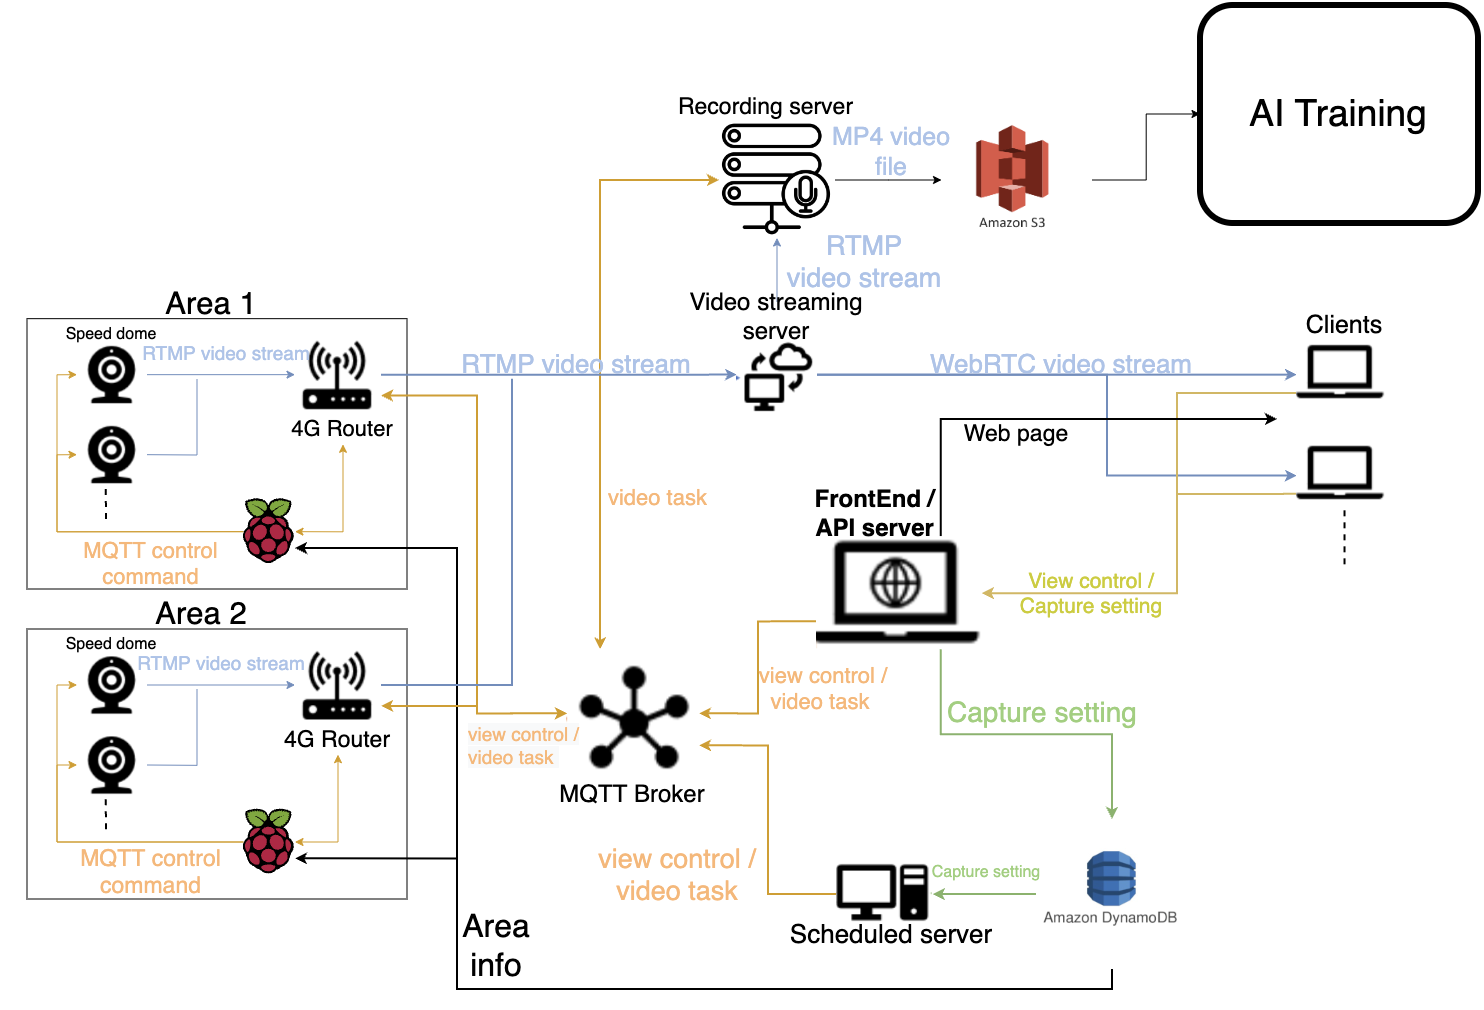
\includegraphics[width=\textwidth]{figsrc/big-system.png}
    \caption{Schematic diagram of system\label{fig:big-system}}
\end{figure}

\section{Smart farm platform}
Smart Farming Platform~\cite{agri-web} is established by National Tsing Hua University High Speed Network Lab(HSNL). HSNL installed sensor and camera on site in order to capture data such as image, live stream, soil moisture or any other sensor data. Process data and upload it to platform then show on webpage for expert to analyze or use as training data set for AI model. Also, users are able to update their farming log to preserve critical information and recieve important message by LINE notifications~\cite{line-notify} from platform. Although it has the ability to capture images, it cannot record video for advanced training. Our system is integrated into this platform to execute recording tasks.

% 下面講每個components在幹麼
\section{Components explanation}
Here, we will discribe what each component are responsible for.
    % local 場域
\subsection{Speed dome}
Speed dome~\cite{speed-dome} is a Pan/Tilt/Zoom(PTZ) doom camera bought in hertone company~\cite{hertone-LTD} as shown in Fig.~\ref{fig:speeddome}. User can control camera remotely by API calling. It has such wide vision that it can rotate 180 degree vertically and 360 degree horizontally. It can push RTMP streaming to server and has night vision. For video quality perspective, it has resolution of 1920x1080 and frame per second(FPS) of 30. At last, user can adjust camera to a special angle and store the angle as preset. If user wants to rotate to that special angle next time, it only need to call API to command camera to rotate automatically. This is one of the main feature for our recording system.
\begin{figure}[H]
    \centering
    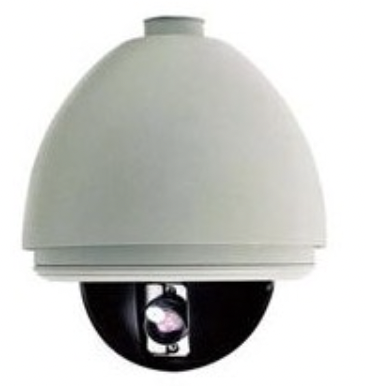
\includegraphics[width=\textwidth / 3]{figsrc/speeddome.png}
    \caption{Speed dome camera\label{fig:speeddome}}
\end{figure}

%     PI
\subsection{Raspberry PI}
Raspberry Pi~\cite{pi} is a series of small single-board computers which is cheaper than standard personal computer as shown in Fig.~\ref{fig:pi}. It is placed in experimental field with Speed dome. PI acts as a edge management device. It recieves command from other servers by MQTT~\cite{mqtt-intro} protocol then commands camera by API request and sends recording request Recording server to execute. Spec of CPU is Quad core, ARM Cortex-A72(v8) 64bytes 1.5GHz and RAM is 4GB LPDDR4-2400 SDRAM and storage is 16 GB MicroSD.

\begin{figure}[H]
    \centering
    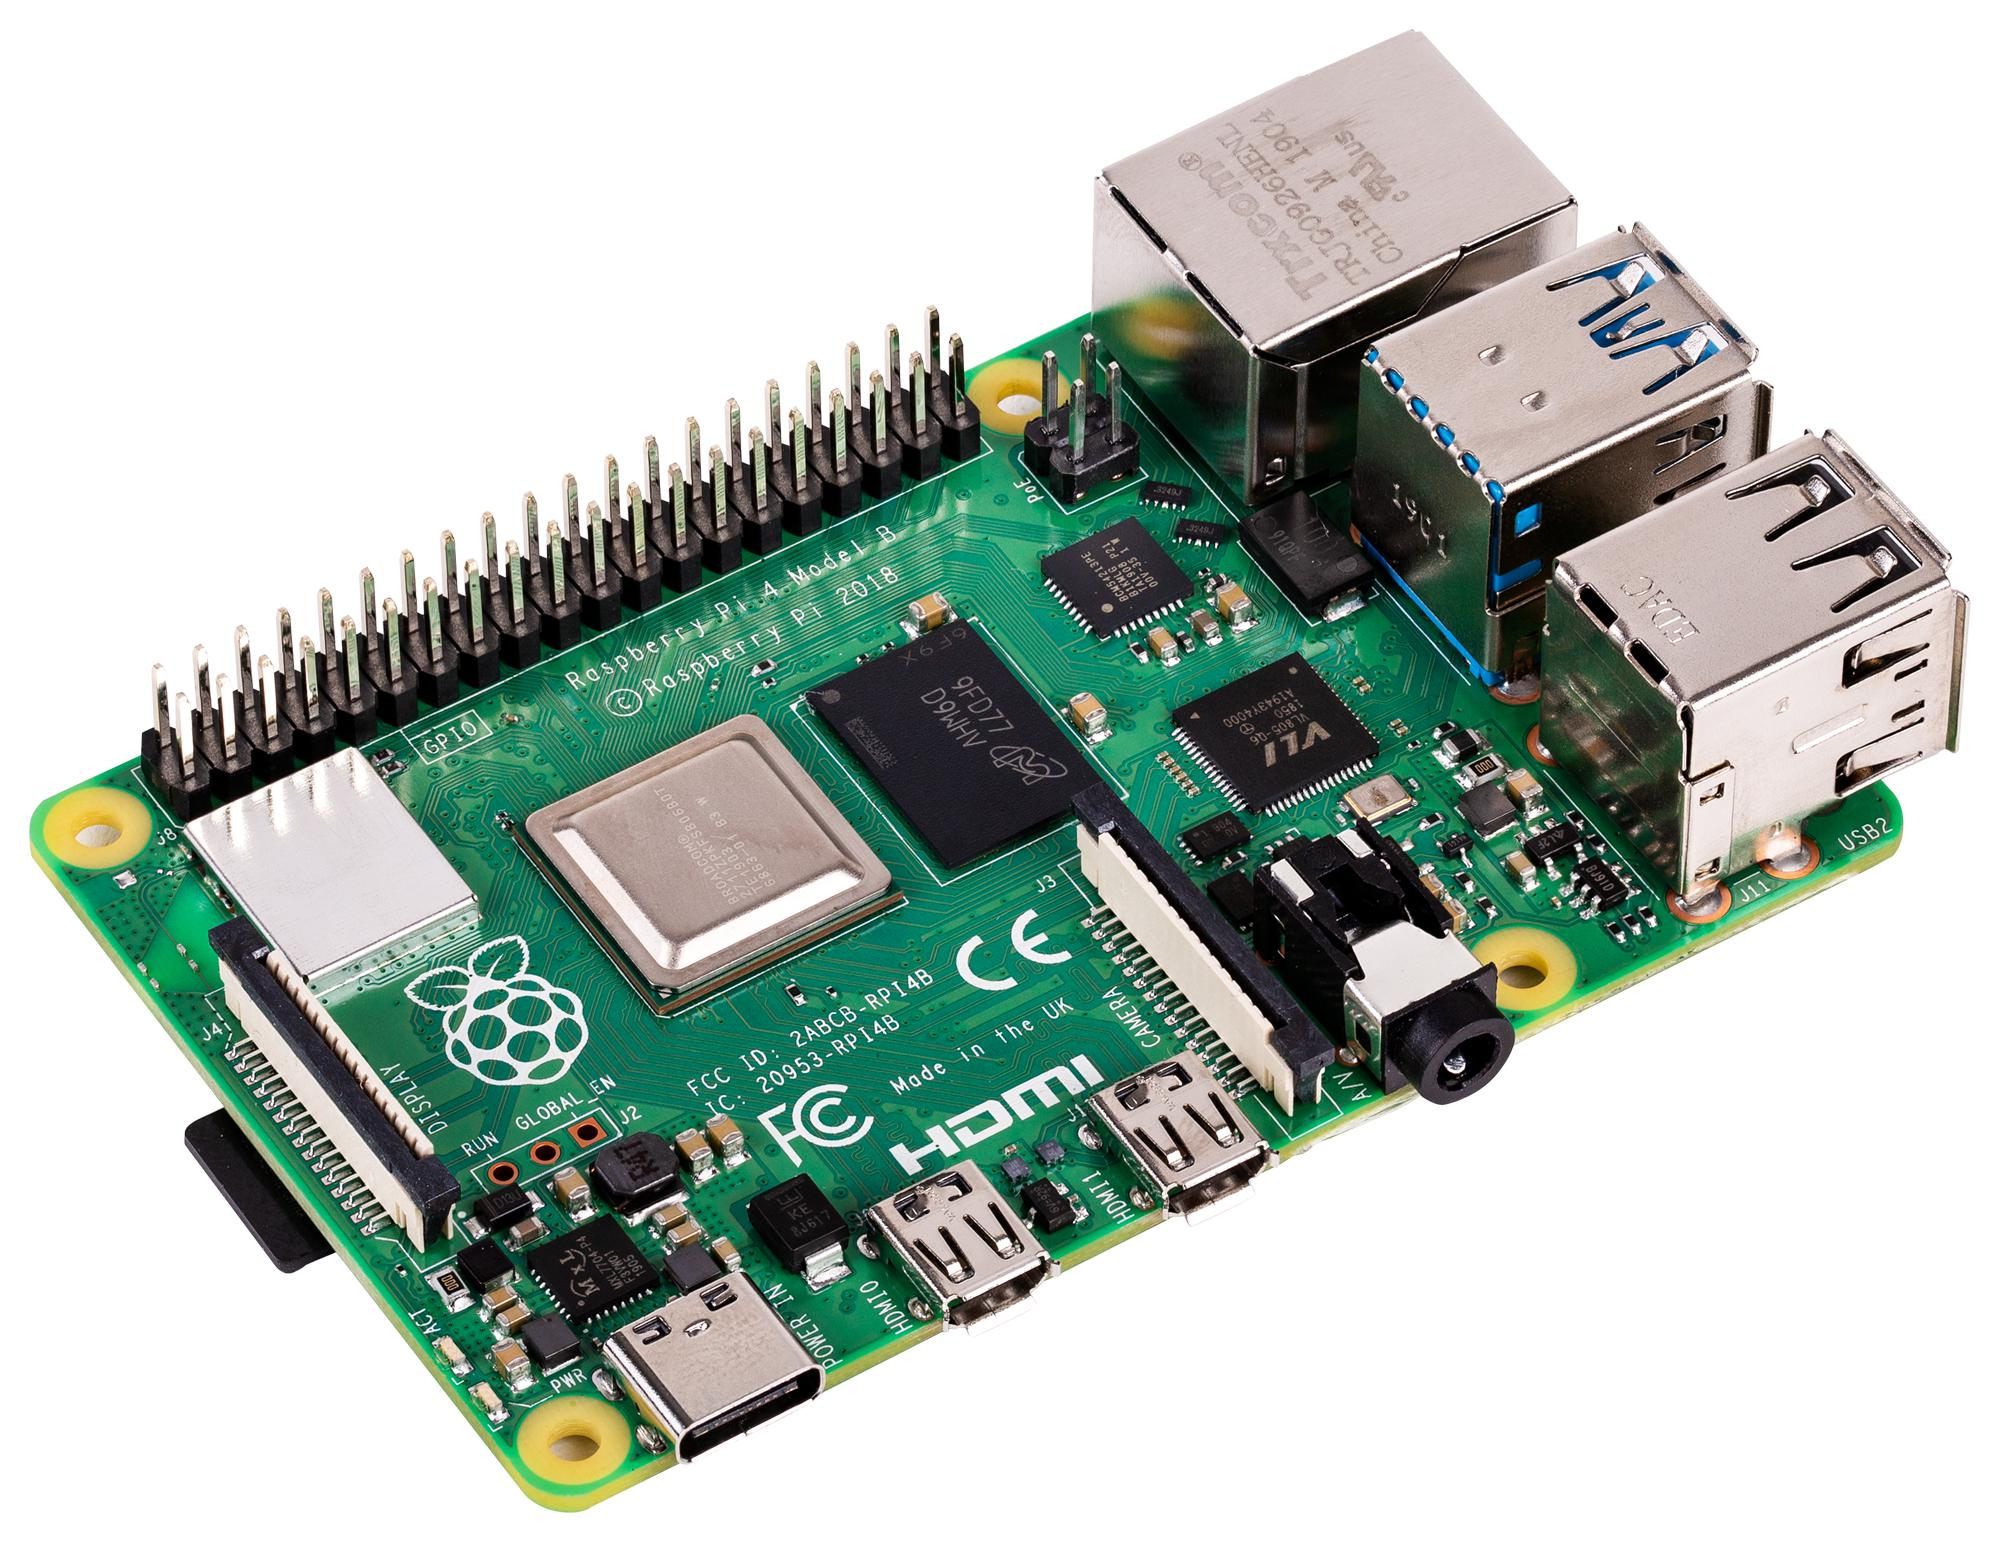
\includegraphics[width=\textwidth]{figsrc/pi.jpeg}
    \caption{Raspberry PI\label{fig:pi}}
\end{figure}

%     % 網路端
%     Video streaming server
\subsection{Video streaming server}
Video streaming server~\cite{ossr} is open sourcing streaming server. It is a simple, high efficiency and realtime video server, supports RTMP/WebRTC/HLS/HTTP-FLV/SRT. It is used to recieve RTMP streaming from Speed dome.

%     recording server
\subsection{Recording server}
Recording server receives command from PI. It is reponsible for pulling live streaming from Video streaming server then turns into video file. After server finish recording, it uploads file to AWS S3. Our recording process uses the feature of OpenCV~\cite{opencv} as our backbone. It has some advantages such as easy to use, supporting multi stream protocol(RTMP, RTSP …etc.) and less bug.

%     API server
%     Front end
%     aws s3
%     aws dynamoDB
\subsection{File Storage and Database}
We utilize AWS S3 to store video file and AWS DynamoDB~\cite{aws-dynamodb} as database. DynamoDB will store various metadata, including scheduled time for recording, meta data for PI in edge side.

%     scheduled server
\subsection{Scheduling server}
Scheduling server fetches information from DynamoDB and is responsible for sending recording request to PI when some events or specific timing occured.


%     MQTT broker 
\section{User cases enumeration}
Here, we will show the user cases for our system. We explain how our system works through sequence diagram for each user case.
% 這邊列舉3個user case
% manual
\subsection{Manual case}
In this user case, User will click the recording button in the streaming web page to manually start recording as shown in Fig.~\ref{fig:manual-case}. 


\begin{figure}[H]
    \centering
    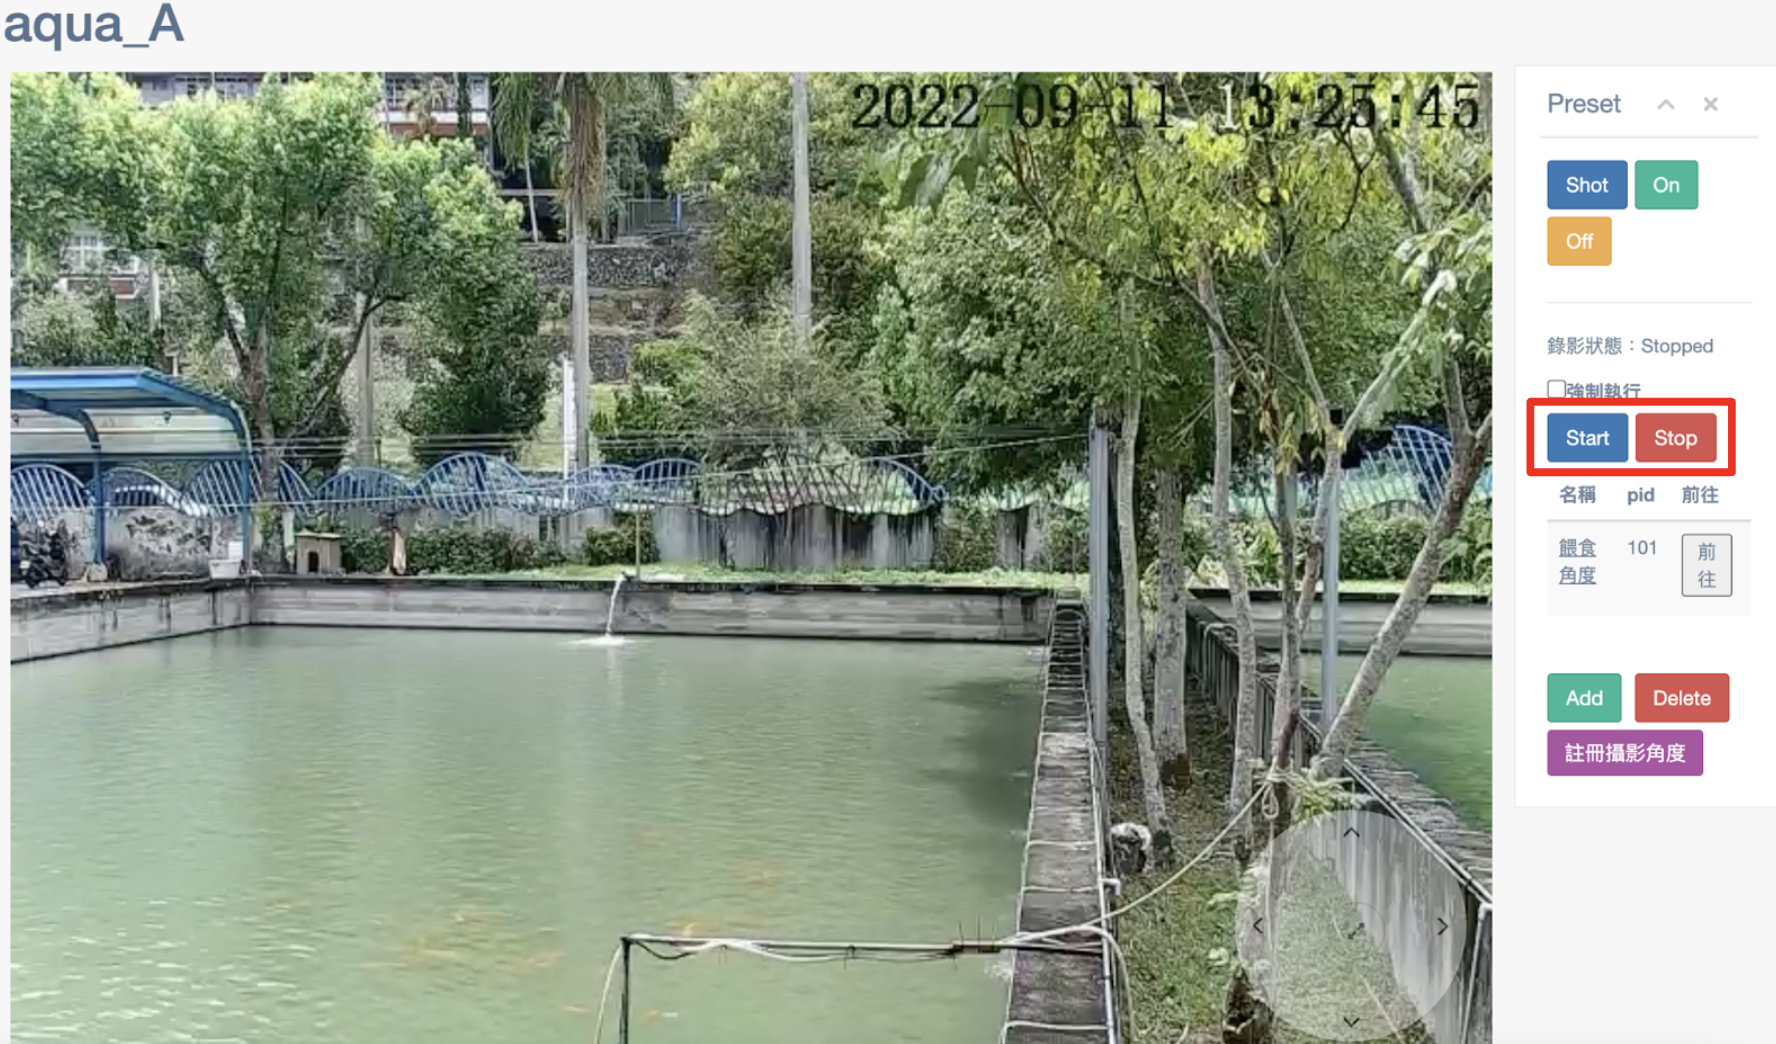
\includegraphics[width=\textwidth]{figsrc/manual-case.png}
    \caption{Click start button to start recording and Press stop button to stop\label{fig:manual-case}}
\end{figure}

As shown in Fig.~\ref{fig:manual-sequece-diagram}, we show the data flow of the whole system from starting the recording task to terminating it. In this manual case, there are 5 components involved, Front-end server, API server(Back-end server), Raspberry PI, Recording server and Video streaming server. When Front-end server sends API request, Back-end will query PI for the permission of the camera. If PI allows the request, it will inform Back-end server that it is ready to recieve recording request. Front-end will recieve permission response from Back-end then start to initiate WebSocket~\cite{websocket} connection with Back-end. After WebSocket connection is complete, Back-end will send MQTT recording command to PI to start recording process. PI will inform Recording server to start connection with Video streaming server and wait until the connection is complete. Recording server will inform PI that connection is complete then PI will inform Recording server to start recording. At the same time, PI will also inform Front-end that the recording process has started. If user wants to terminate the recording task, he/she can press the stop button. Front-end will disconnect WebSoceket. When Back-end detect WebSocket connection has been shut down, it will send stop command to inform PI to stop the process. At last, Recording server will stop connection with Video streaming server then upload the video file to AWS S3~\cite{aws-s3}.

\begin{figure}[H]
    \centering
    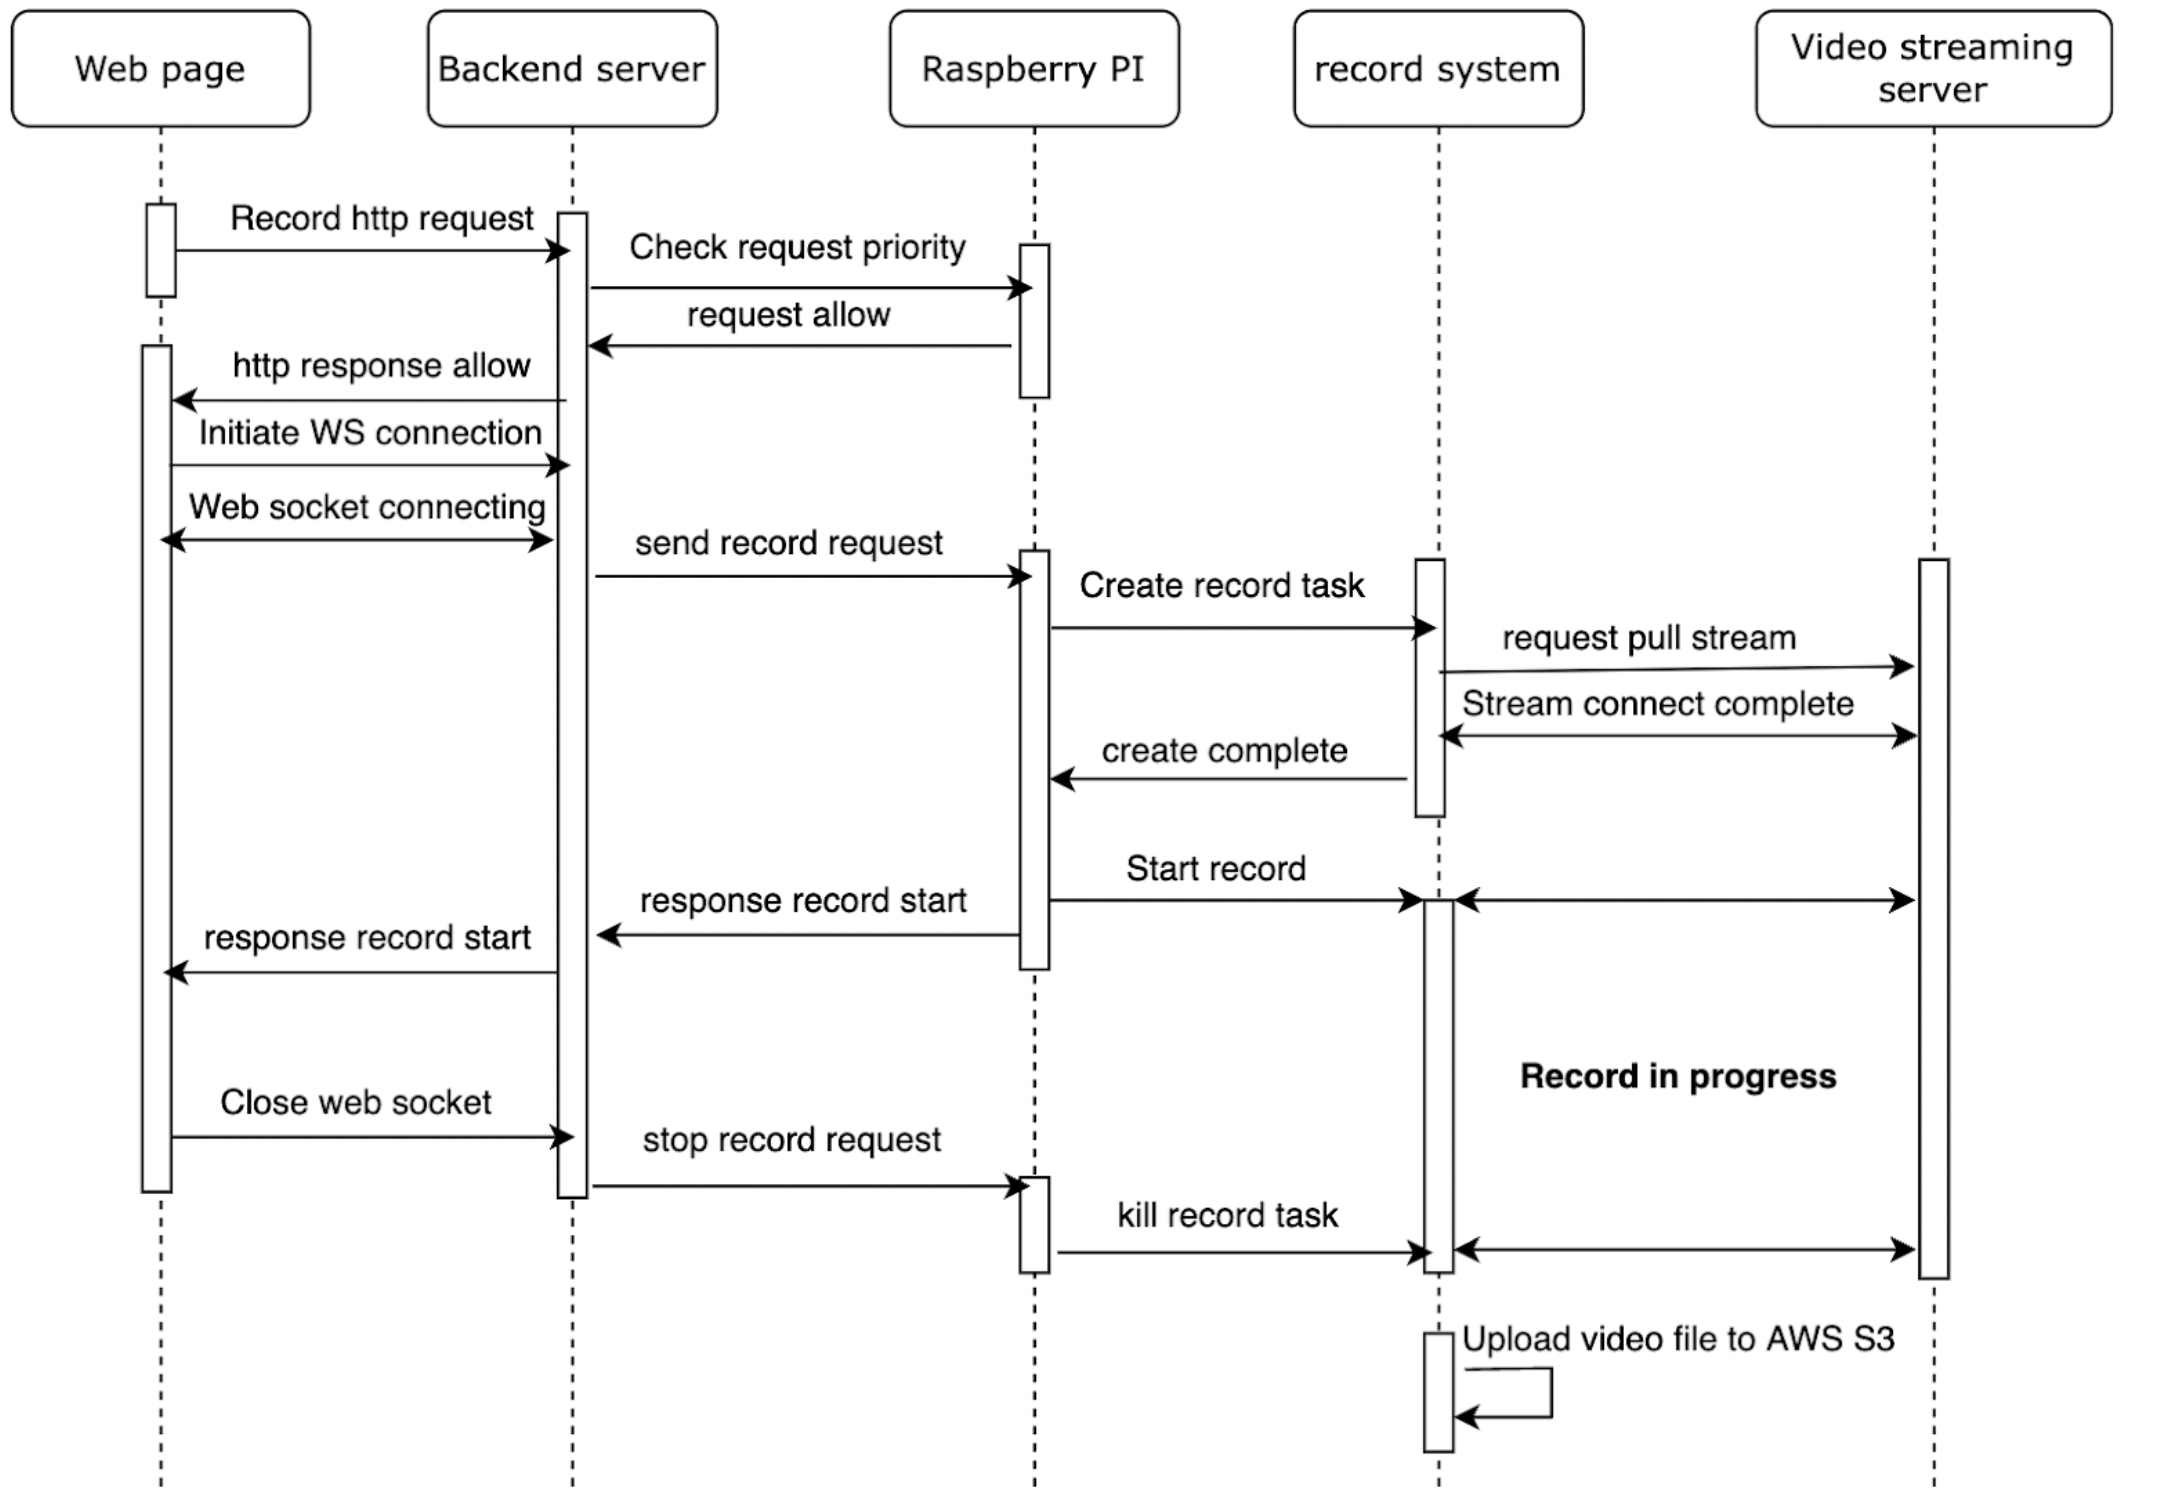
\includegraphics[width=\textwidth]{figsrc/manual-sequece-diagram.png}
    \caption{Data flow of manual case\label{fig:manual-sequece-diagram}}
\end{figure}

% event
\subsection{Event triggered case}
In this case, recording process will start if specific event occured. Users have to register the event they want(e.g. Some sensor value exceed specific threshold.) to record. The steps are shown in Fig.~\ref{fig:event-userflow}. First, in Fig.~\ref{fig:event-userflow-a}, users can rotate camera to the angle they want then press the purple button to store the angle. Second, in Fig.~\ref{fig:event-userflow-b}, They can set a name for this angle. Third, in FIg.~\ref{fig:event-userflow-c}, They will set the recording duration, angle name, the type of event.

\begin{figure}[H]
    \centering
    \begin{subfigure}{\textwidth}
        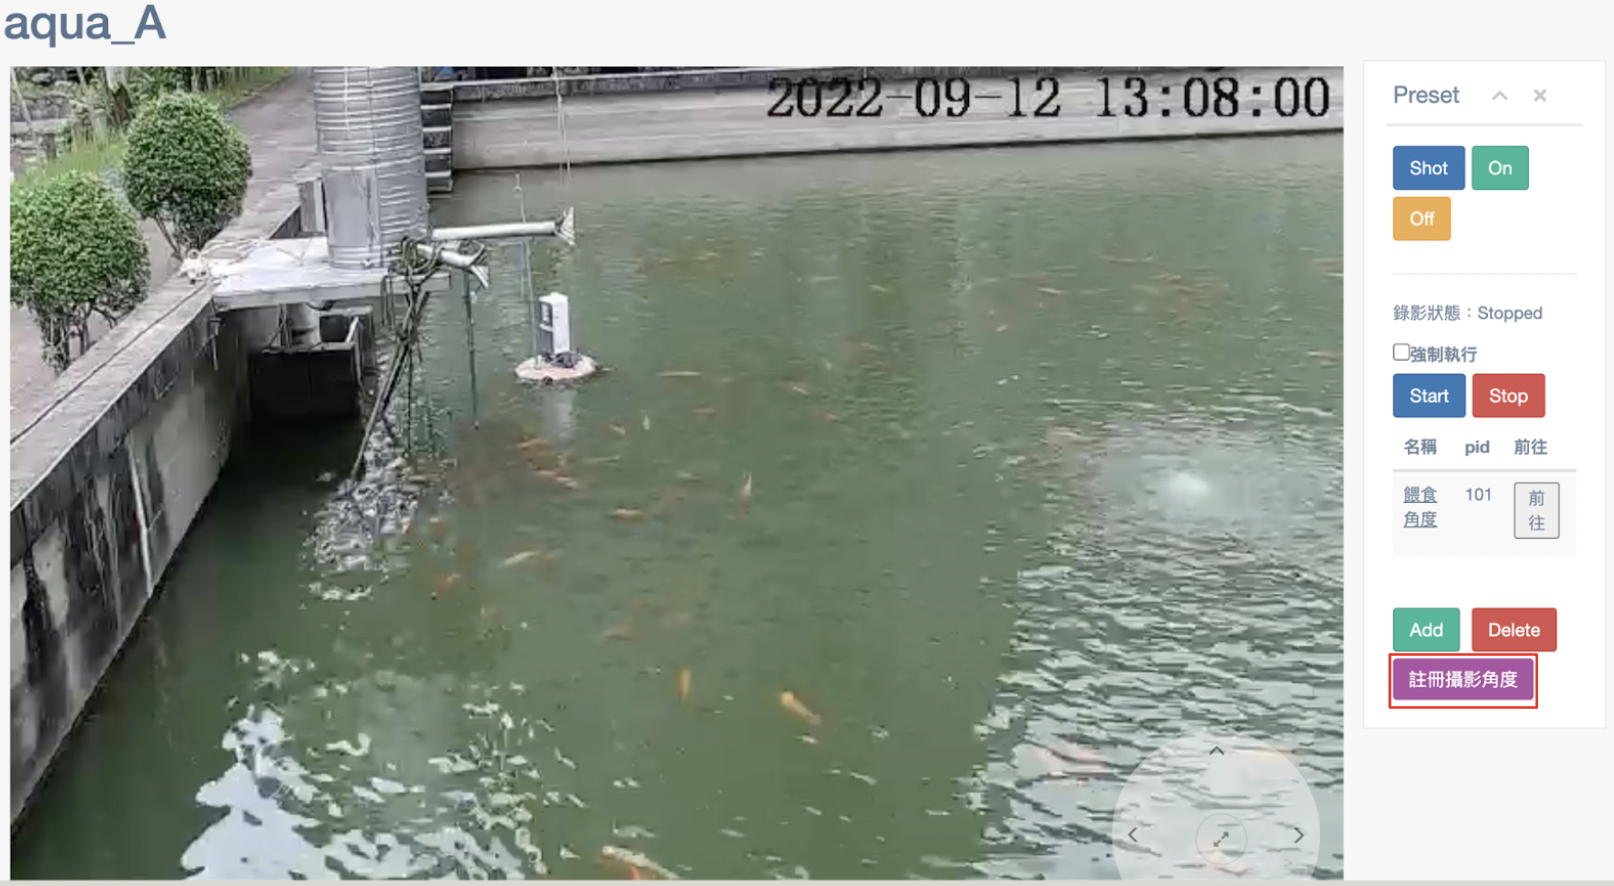
\includegraphics[width=\textwidth]{figsrc/event-userflow-a.png}
        \subcaption{Go to an angle you want}
        \label{fig:event-userflow-a}
    \end{subfigure}

\medskip
    \begin{subfigure}{\textwidth}
        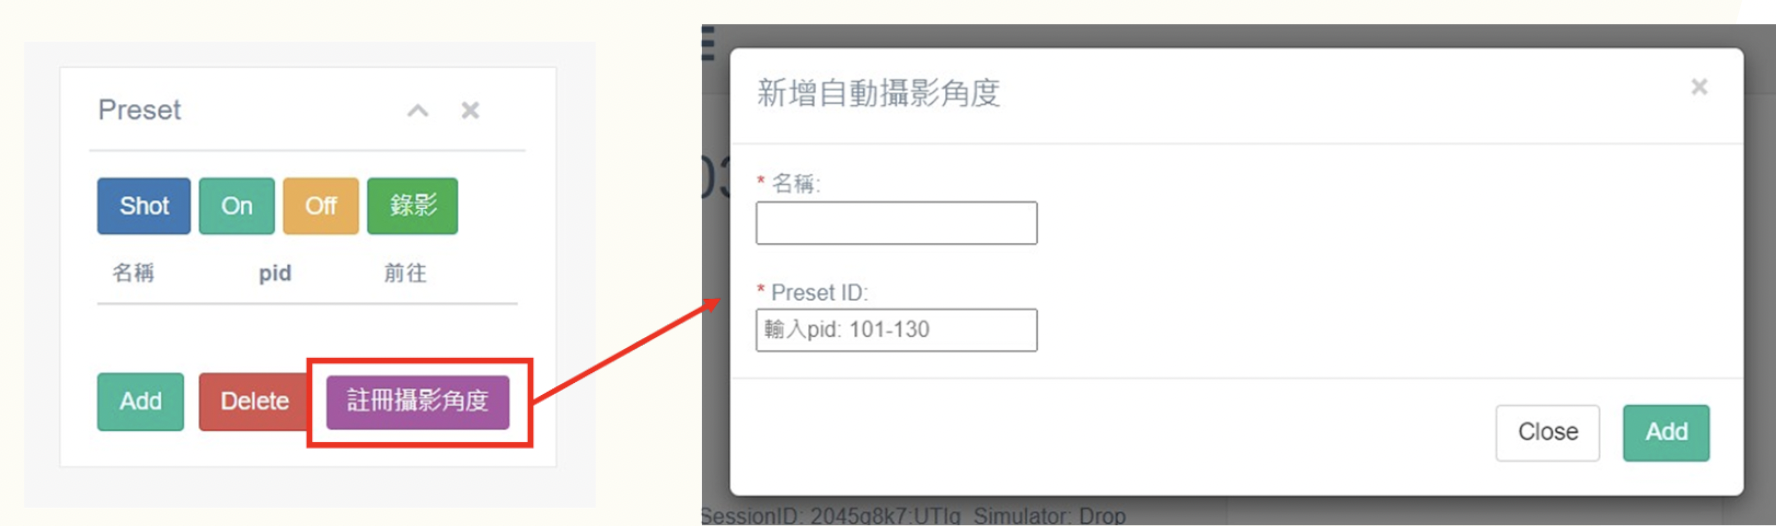
\includegraphics[width=\textwidth]{figsrc/event-userflow-b.png}
        \subcaption{Set a name for this angle}
        \label{fig:event-userflow-b}
    \end{subfigure}
    \caption{User flow of event triggered case}
\end{figure}

\begin{figure}[H]
    \ContinuedFloat
    \centering
    \begin{subfigure}{\textwidth}
        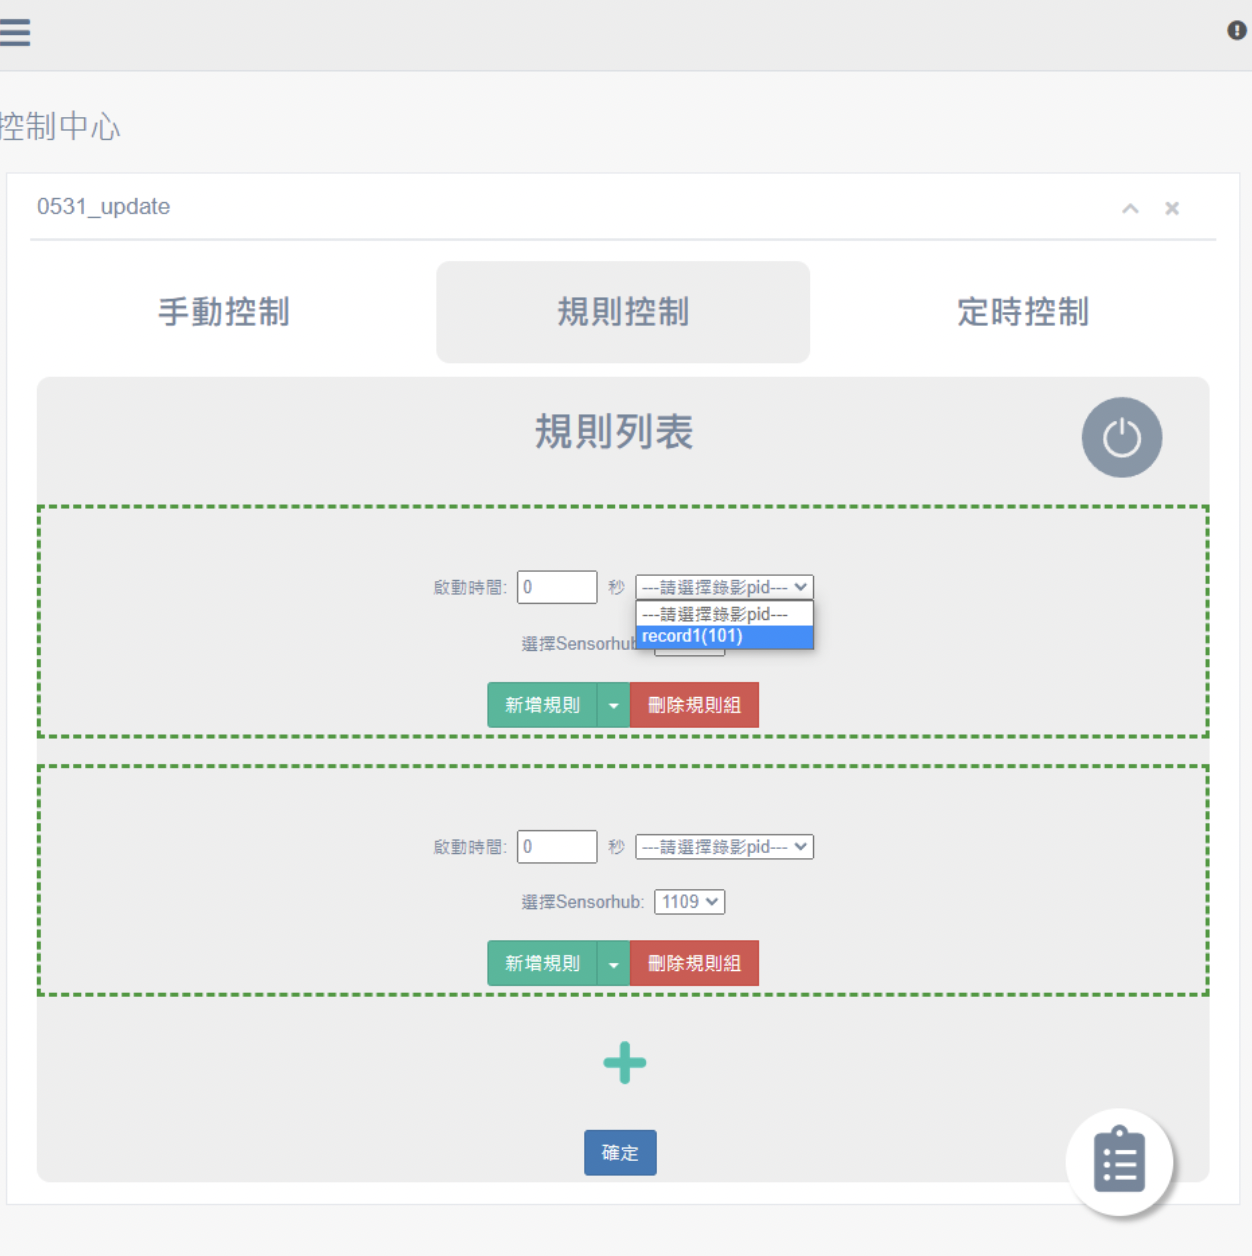
\includegraphics[width=\textwidth]{figsrc/event-userflow-c.png}
        \subcaption{Choose an event}
        \label{fig:event-userflow-c}
    \end{subfigure}

    \caption{User flow of event triggered case(cont.)}
    \label{fig:event-userflow}
\end{figure}

We will also show the sequence diagram of event case below from registering event to recording process terminated in Fig.~\ref{fig:event-sequence-diagram}. In this case, there are 6 components involved, Front-end server, API server(Back-end server), Scheduling server, Raspberry PI, Recording server and Video streaming server. When user registers a event, Back-end will send the event information, including camera angle, recording duration and task type, to scheduling server. When event occured, scheduling server will send recording request to Recording server. Similar to manual case, PI will inform Recording server to start connection with streaming server and wait until the connection is complete. Recording server will inform PI that connection is complete then PI will inform Recording server to start recording for X seconds. Recording server will shut down video process when time's up. At last, Recording server will stop connection with Video streaming server then upload the video file to AWS S3.

\begin{figure}[H]
    \centering
    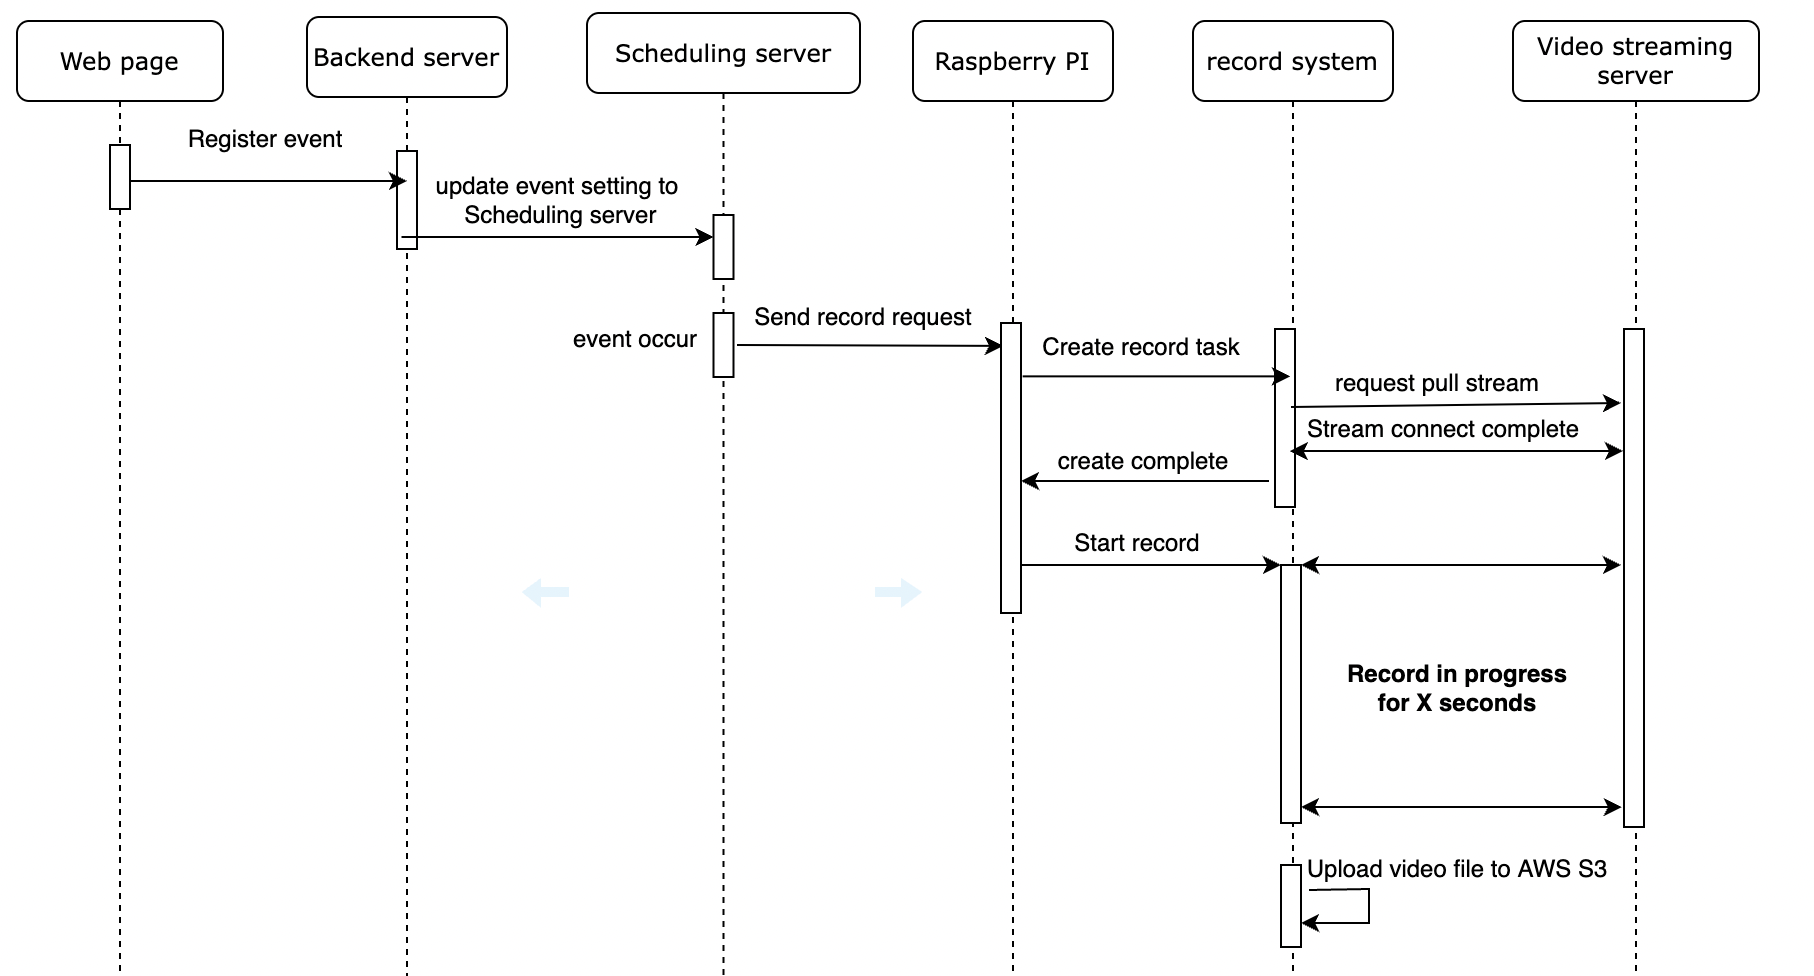
\includegraphics[width=\textwidth]{figsrc/event-sequence-diagram.png}
    \caption{Data flow of event triggered case\label{fig:event-sequence-diagram}}
\end{figure}


% time
\subsection{Time period triggered case}
In this case, recording process will be triggered at a specific timing. Similar to event register, as shown in Fig.~\ref{fig:time-userflow-a}, users can rotate camera to the angle they want then press the purple button to store the angle, then in Fig.~\ref{fig:time-userflow-b} users can set a name for this angle. At last, in Fig.~\ref{fig:time-userflow-c}, They can set the time period, recording duration and recording angle.

\begin{figure}[H]
    \centering
    \begin{subfigure}{\textwidth}
        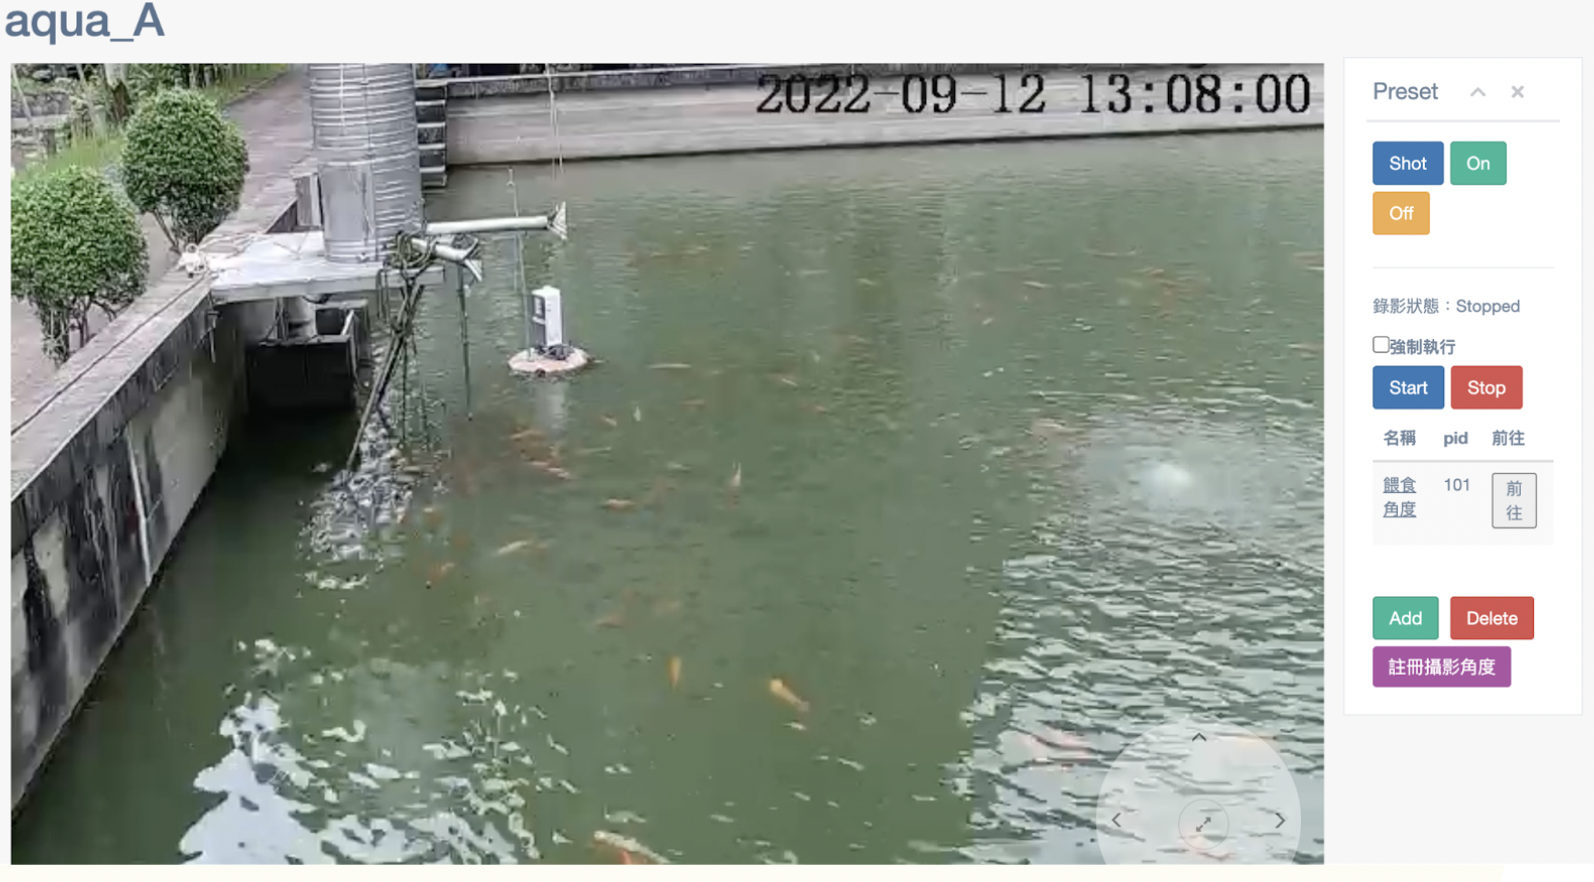
\includegraphics[width=\textwidth]{figsrc/time-userflow-a.png}
        \subcaption{Go to an angle you want}
        \label{fig:time-userflow-a}
    \end{subfigure}

\medskip
    \begin{subfigure}{\textwidth}
        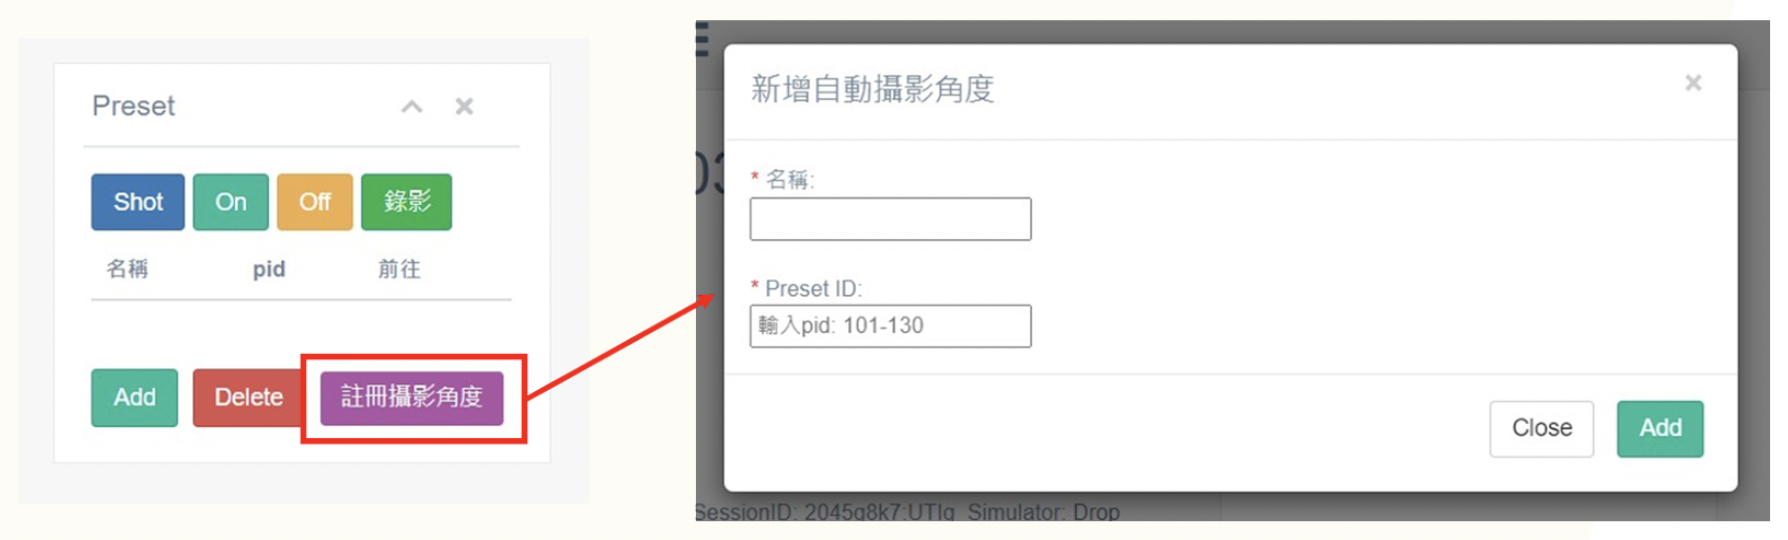
\includegraphics[width=\textwidth]{figsrc/time-userflow-b.png}
        \subcaption{Set a name for this angle}
        \label{fig:time-userflow-b}
    \end{subfigure}
    \caption{User flow of time period triggered case}
\end{figure}

\begin{figure}[H]
    \ContinuedFloat
    \centering
    \begin{subfigure}{\textwidth}
        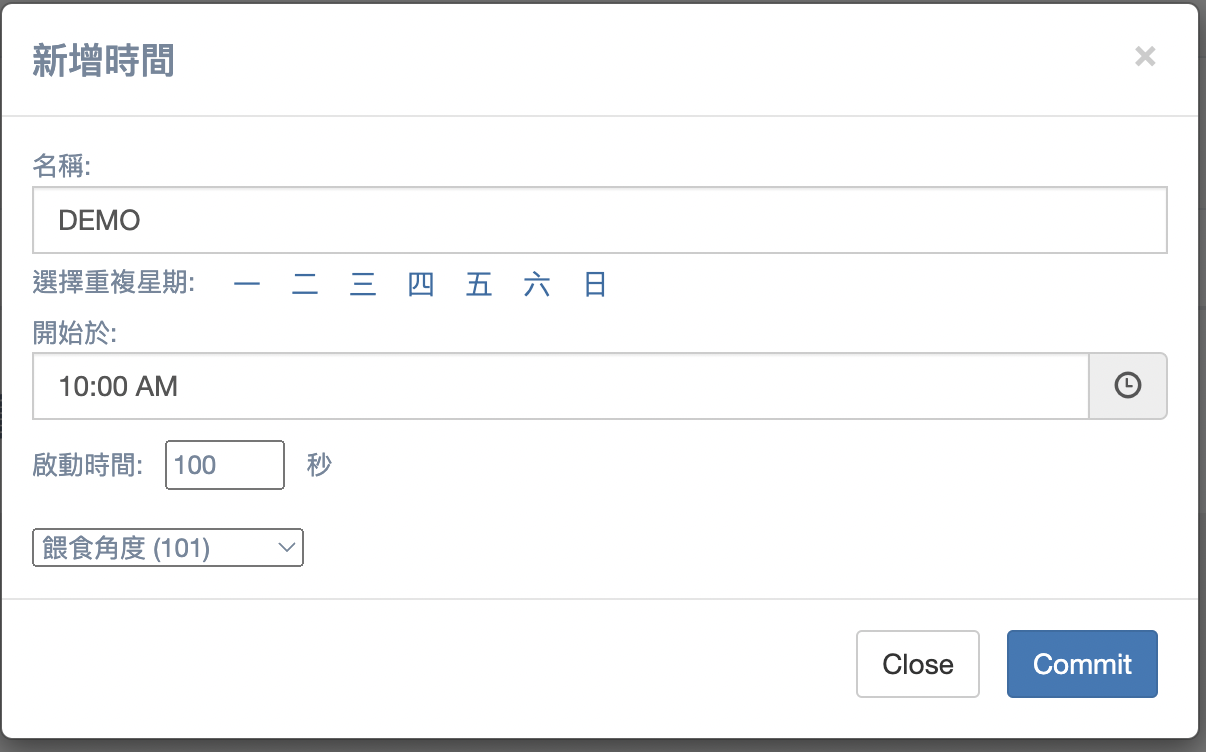
\includegraphics[width=\textwidth]{figsrc/time-userflow-c.png}
        \subcaption{Choose an time}
        \label{fig:time-userflow-c}
    \end{subfigure}

    \caption{User flow of time period triggered case(cont.)}
    \label{fig:time-userflow}
\end{figure}

Similar to event trigger case, it has 6 components, Front-end server, API server(Back-end server), Scheduling server, Raspberry PI, Recording server and Video streaming server. The sequence diagram is shown below. In Fig.~\ref{fig:time-sequence-diagram}, when users reigister time setting, Back-end will update the information whilch is identical to event trigger case except the task ID to schduling server. When the time comes, scheduling server will send recording request to PI then do the exact same process in event triggered case. PI will inform Recording server to start connection with streaming server and wait until the connection is complete. Recording server will inform PI that connection is complete then PI will inform Recording server to start recording for X seconds. Recording server will shut down video process when time's up. At last, Recording server will stop connection with Video streaming server then upload the video file to AWS S3.

\begin{figure}[H]
    \centering
    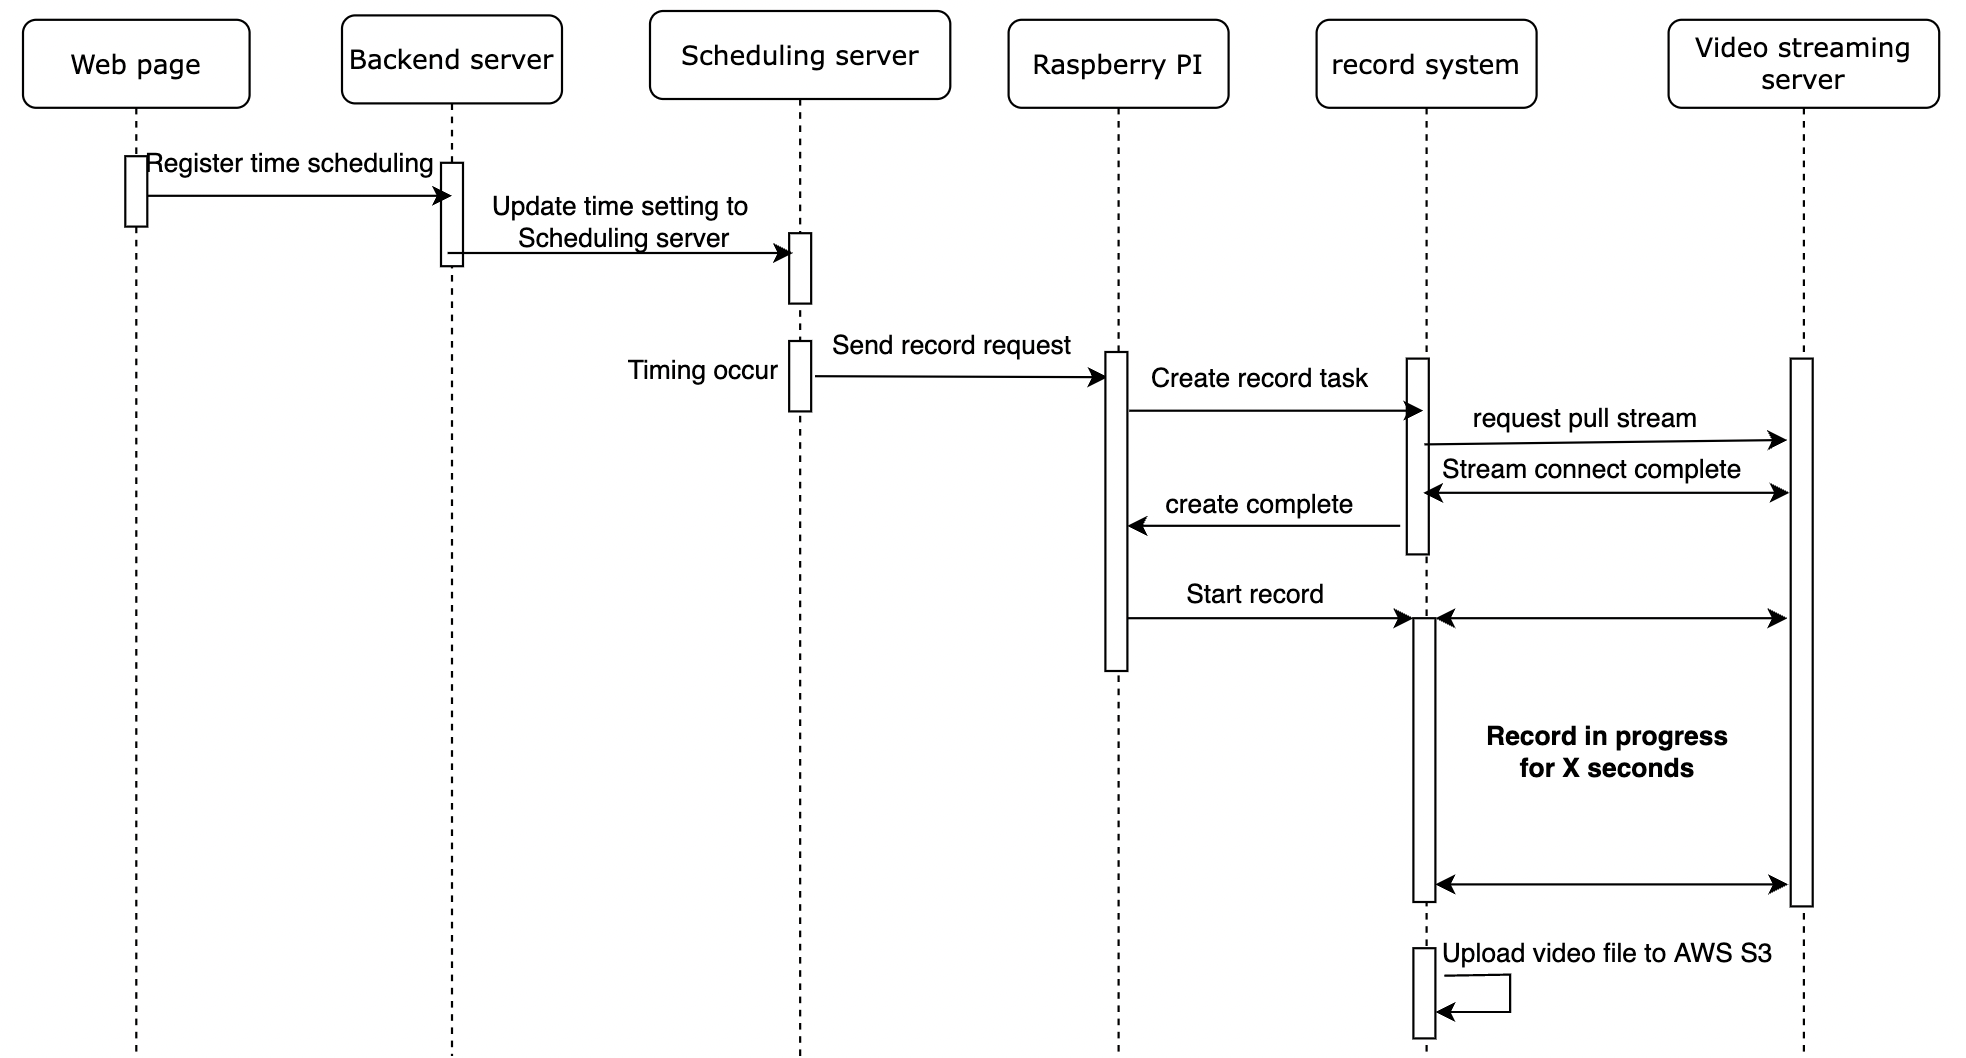
\includegraphics[width=\textwidth]{figsrc/time-sequence-diagram.png}
    \caption{Data flow of time period triggered case\label{fig:time-sequence-diagram}}
\end{figure}

% 1個special case: preemptive
\subsection{Critical case: Preemptive case}
We have shown normal cases that run on our system. Here, we want to point out a special situation. Normally, camera is only capable of executing one recording request. As shown in Fig.~\ref{fig:preemptive-example}, What if there are multiple recording request coming in at the same time?(e.g. At the moment, user A and B want to record manually and an event also triggers the recording process.) It is obvious that camera cannot handle more than one recording request. It doesn't know that which tasks should be executed. We implement priority method to handle such situation in Raspberry PI. If there are multiple tasks, PI can check the importance of each task to decide which task can be executed. For example, PI is running task A. Next, task B comes in and request to record. PI will compare the importance, or prioirty, between task A and B. If B is lower than A, PI will reject the request from B. If B is higher than A, PI will stop task A and turn the permission to task B.


\begin{figure}[H]
    \centering
    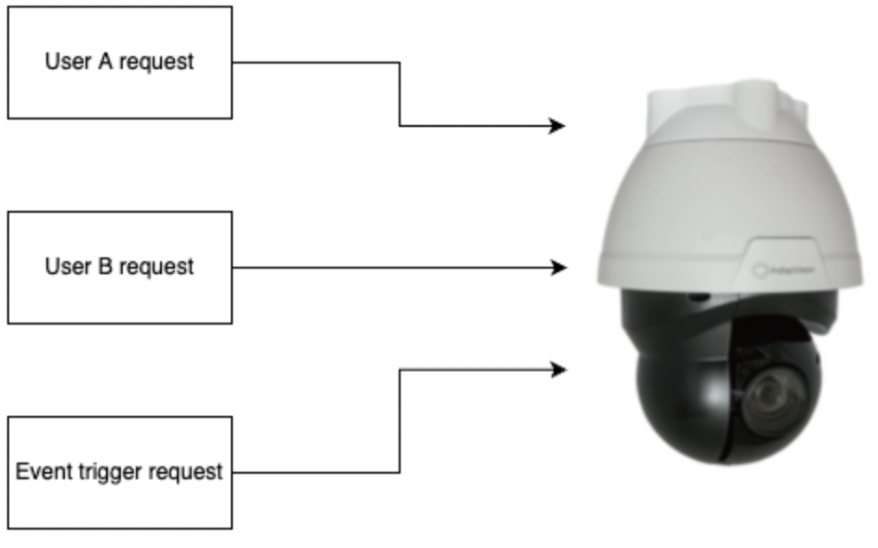
\includegraphics[width=\textwidth]{figsrc/preemptive-example.png}
    \caption{3 requests come at the same time \label{fig:preemptive-example}}
\end{figure}

We will give a preemptive example by showing sequence diagram below. Fig.~\ref{fig:preemptive-a} shows user A requesting recording task at the beginning. PI will execute user A's record as we have shown in maunal case since there are no other tasks yet. Afer Fig.~\ref{fig:preemptive-a}, There will be two cases occured when second user comes in, Fig.~\ref{fig:preemptive-B-higher} and Fig.~\ref{fig:preemptive-B-lower}. Fig.~\ref{fig:preemptive-B-higher} is the case that second user has higher priority and Fig.~\ref{fig:preemptive-B-lower} is the opposite case. 

In Fig.~\ref{fig:preemptive-B-higher} case, user B sends permission checking to PI. PI knows that user A is currently occupying the task, so it checks the priority between A and B. It finds out that B is more important than A, so it returns permission to User B. After user B recieves permission, it starts to build WebSocket connection with Back-end. Back-end sends record command to PI. Since user B have higher priority than user A, PI will order Recording server to stop user A's process. Recording server will stop recording and upload user A's video file then PI will inform Back-end to stop WebSocket connection with User A. User A's web page will recieve a warning from Back-end that the task have been forced to shut down. After PI closes user A's task, it will inform user B that recording task is started and order Recording server to start a new task.

In Fig.~\ref{fig:preemptive-B-lower} case, user B sends permission checking to PI. PI knows that user A is currently occupying the task, so it checks the priority between A and B. It finds out that A is more important than B, so it rejects user B's request and let Recording server keep recording user A's task.

\begin{figure}[H]
    \centering
    \begin{subfigure}{\textwidth}
        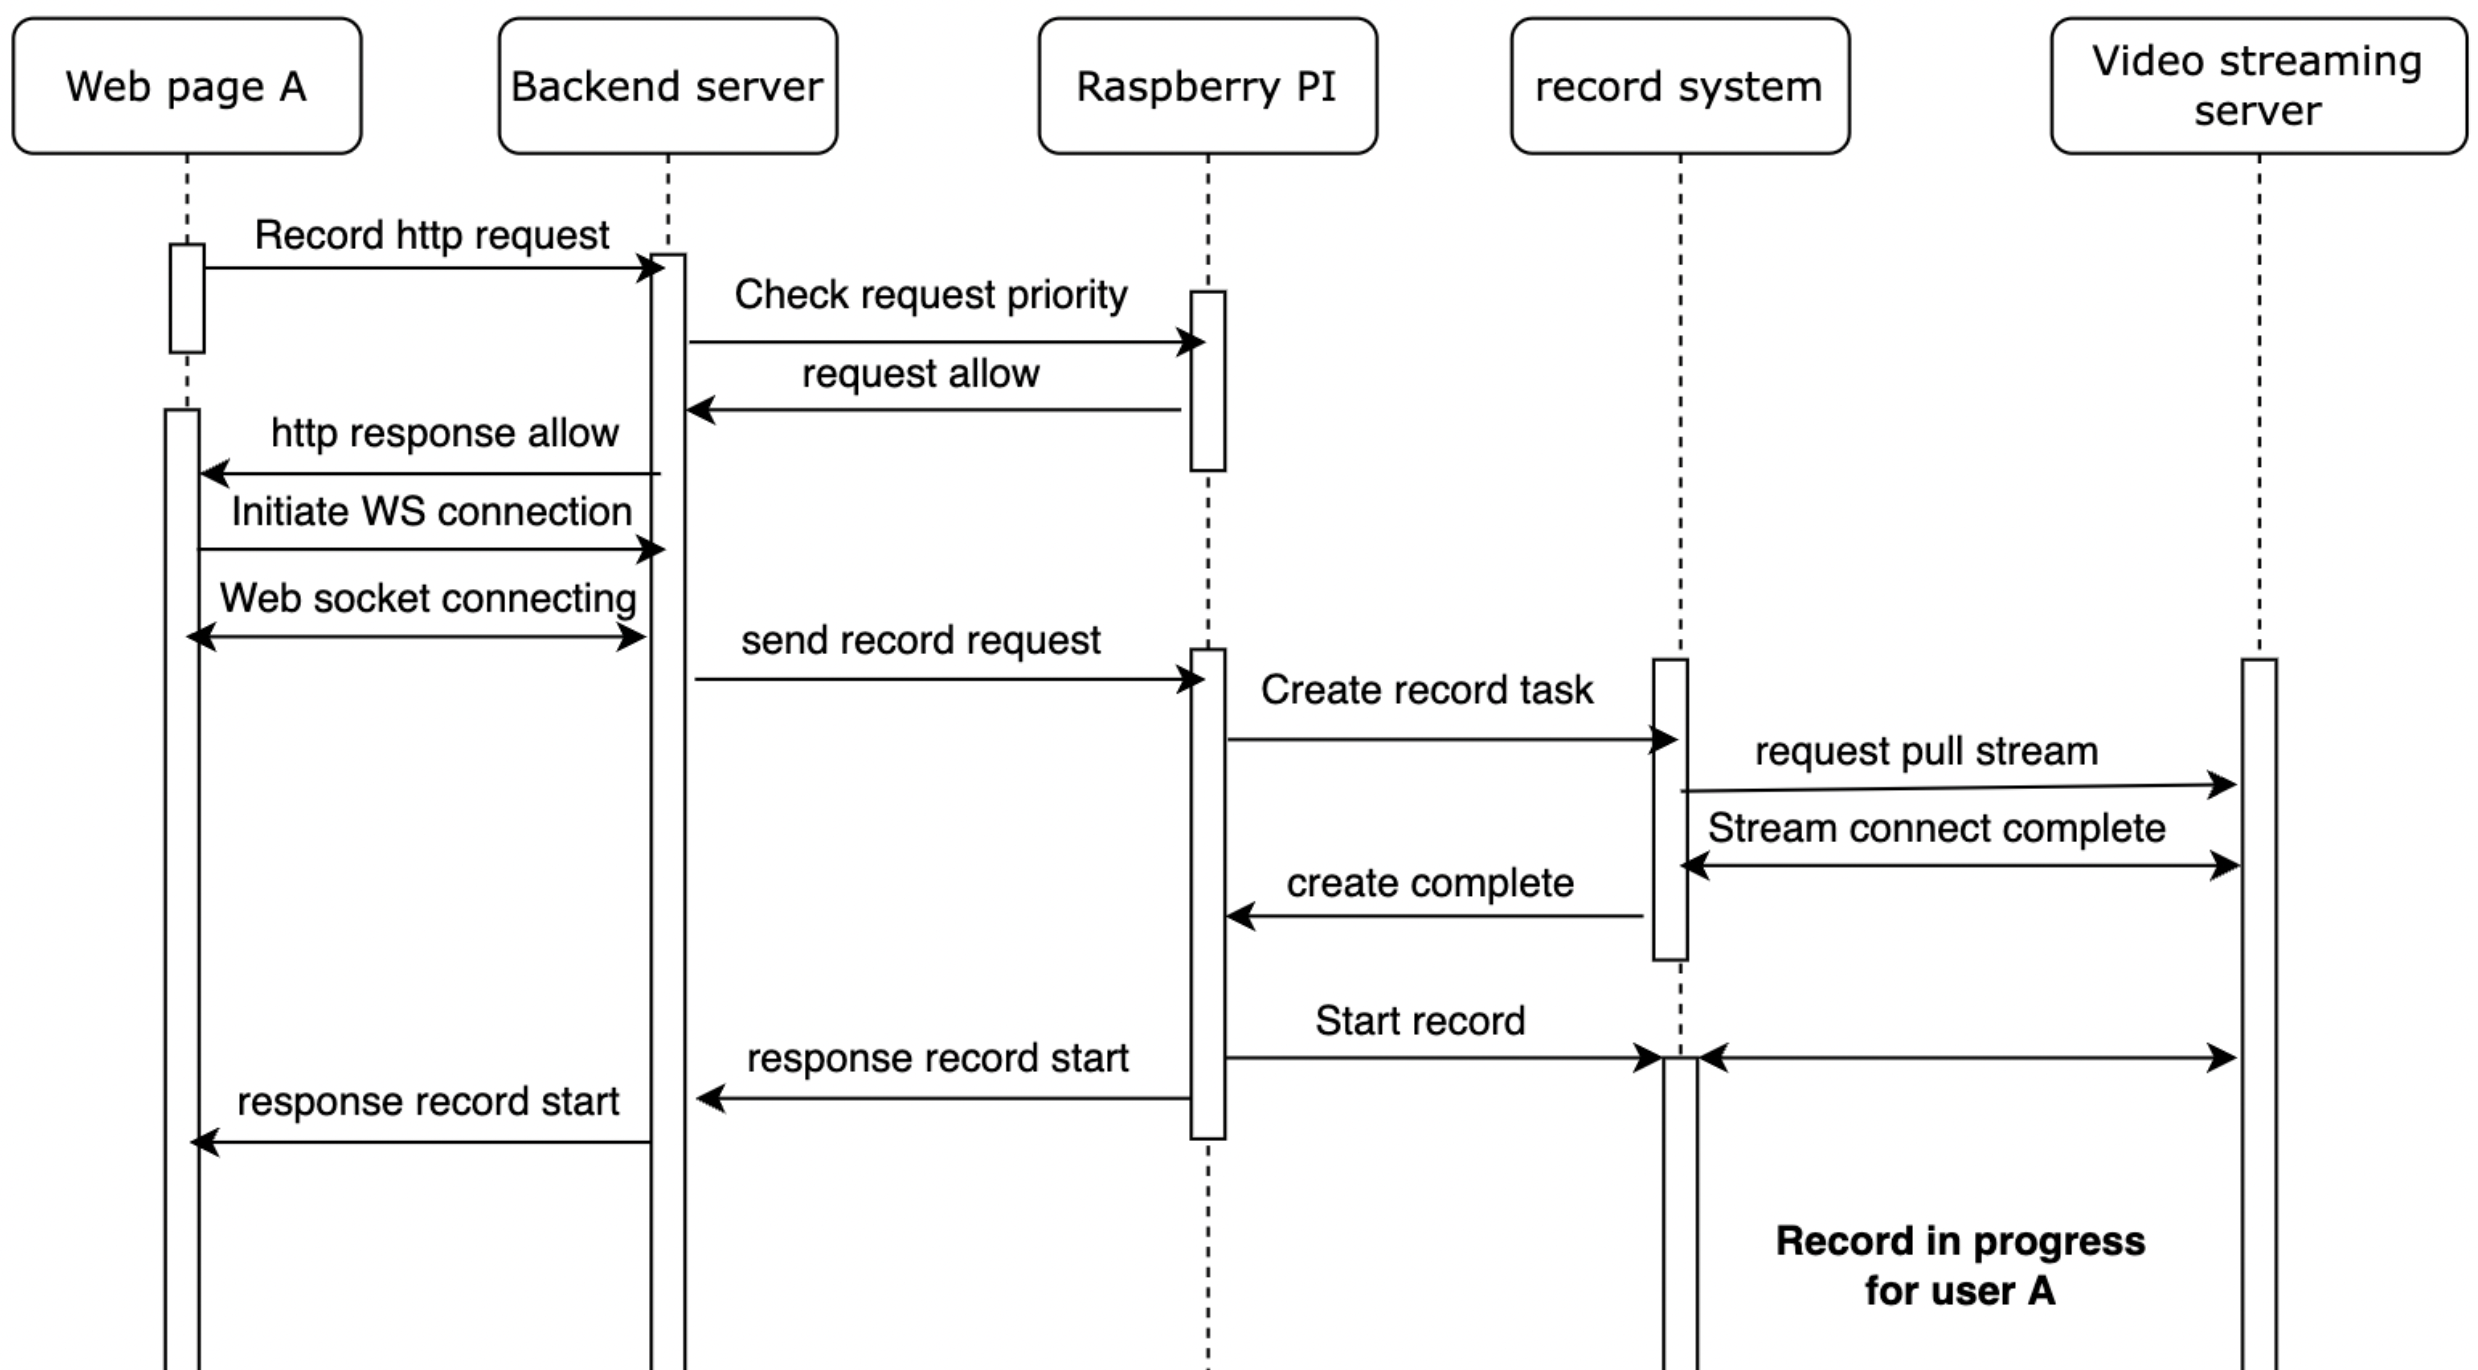
\includegraphics[width=\textwidth]{figsrc/preemptive-a.png}
        \subcaption{User A requests record}
        \label{fig:preemptive-a}
    \end{subfigure}

    % \caption{User flow of time period triggered case(cont.)}
    % \label{fig:time-userflow}
\end{figure}

\begin{figure}[H]
    \ContinuedFloat
    \centering
    \begin{subfigure}{\textwidth}
        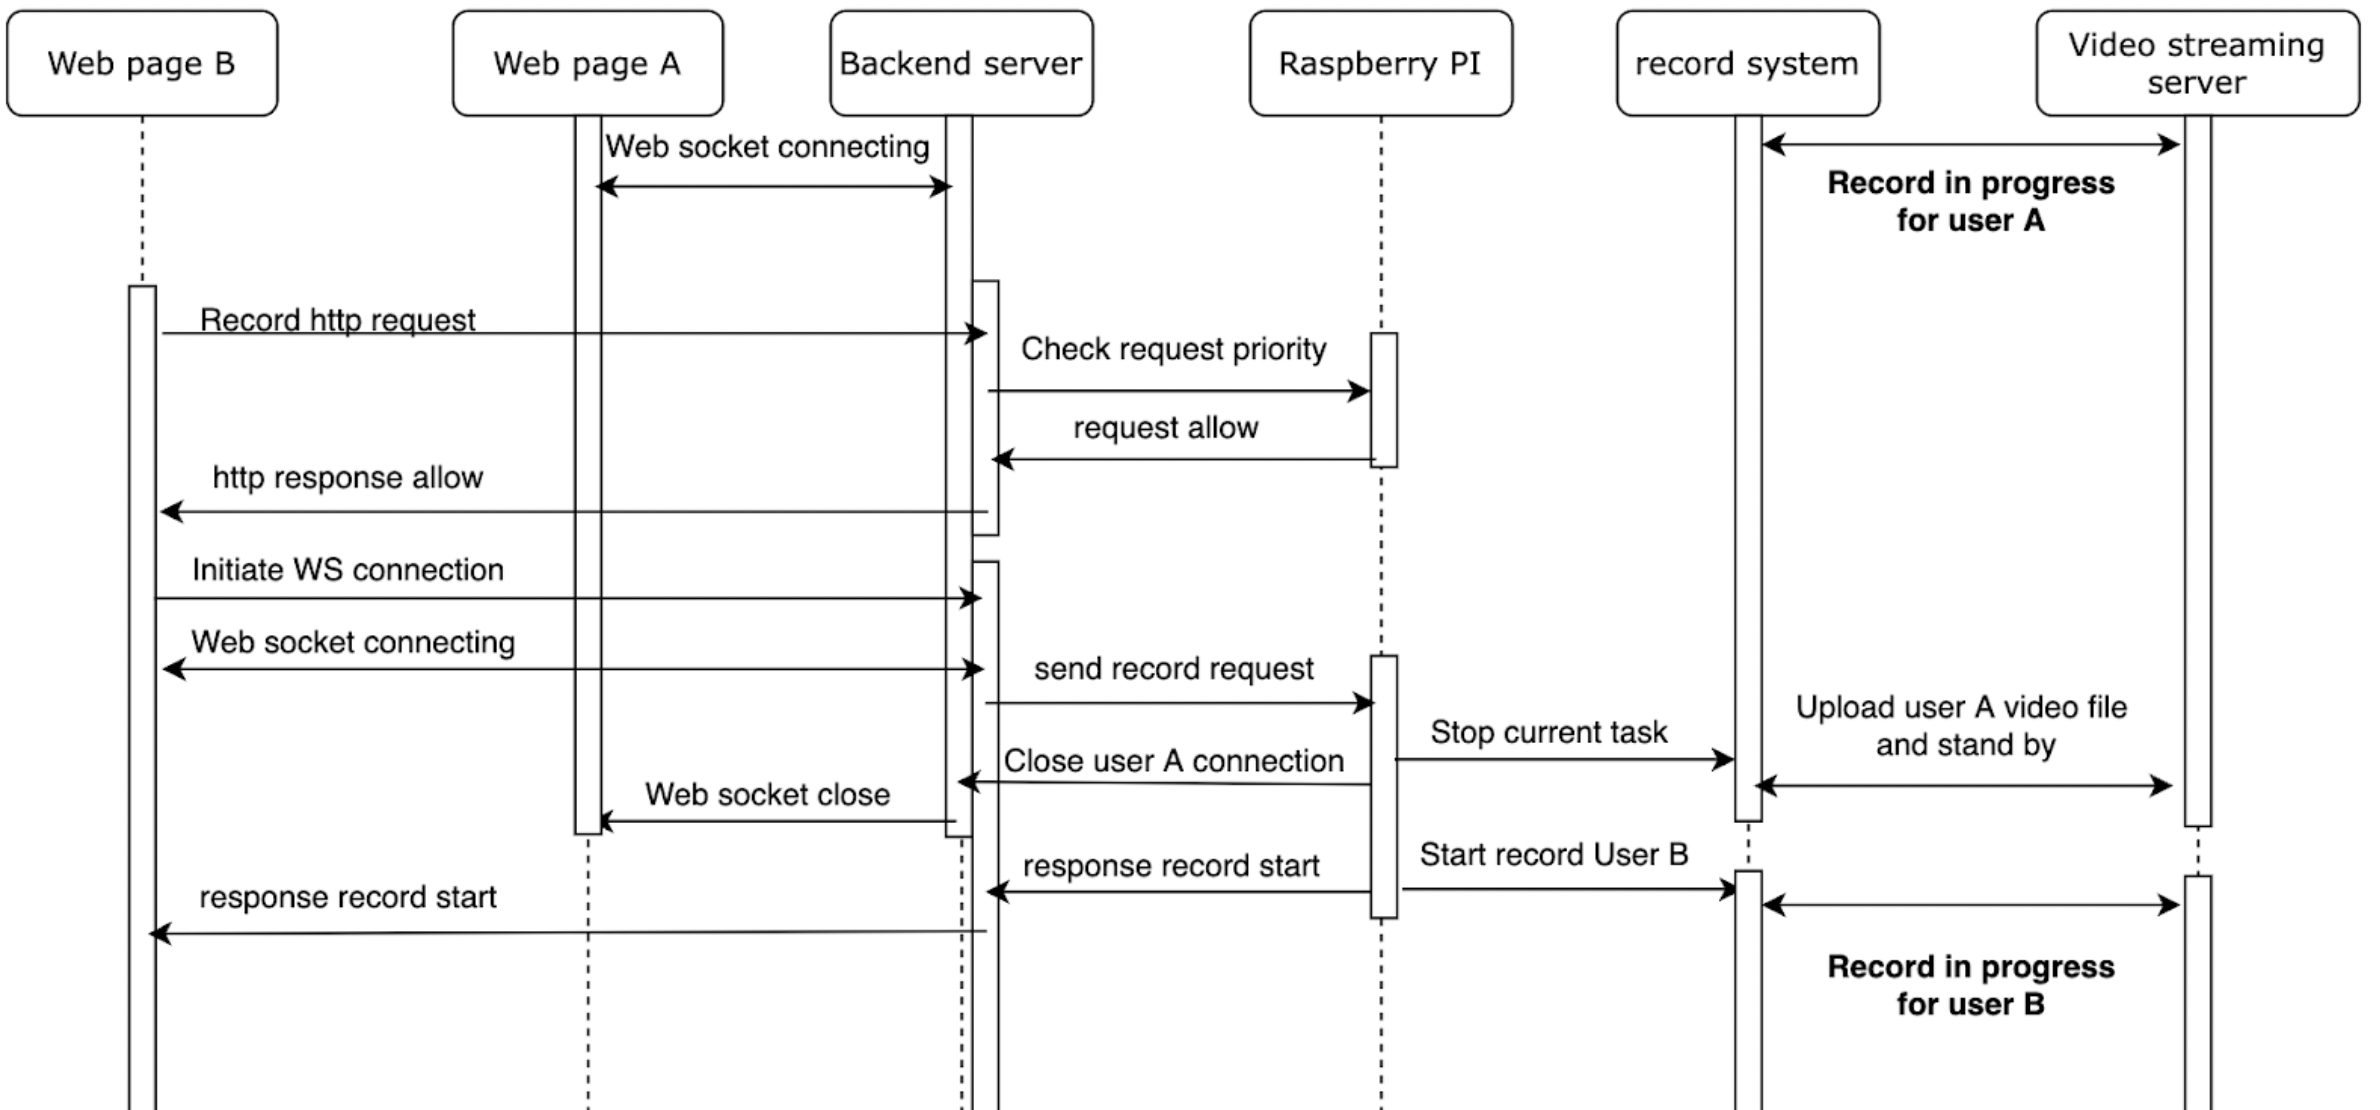
\includegraphics[width=\textwidth]{figsrc/preemptive-B-higher.png}
        \subcaption{User B with higher priority}
        \label{fig:preemptive-B-higher}
    \end{subfigure}

    % \caption{User flow of time period triggered case(cont.)}
    % \label{fig:time-userflow}
\end{figure}

\begin{figure}[H]
    \ContinuedFloat
    \centering
    \begin{subfigure}{\textwidth}
        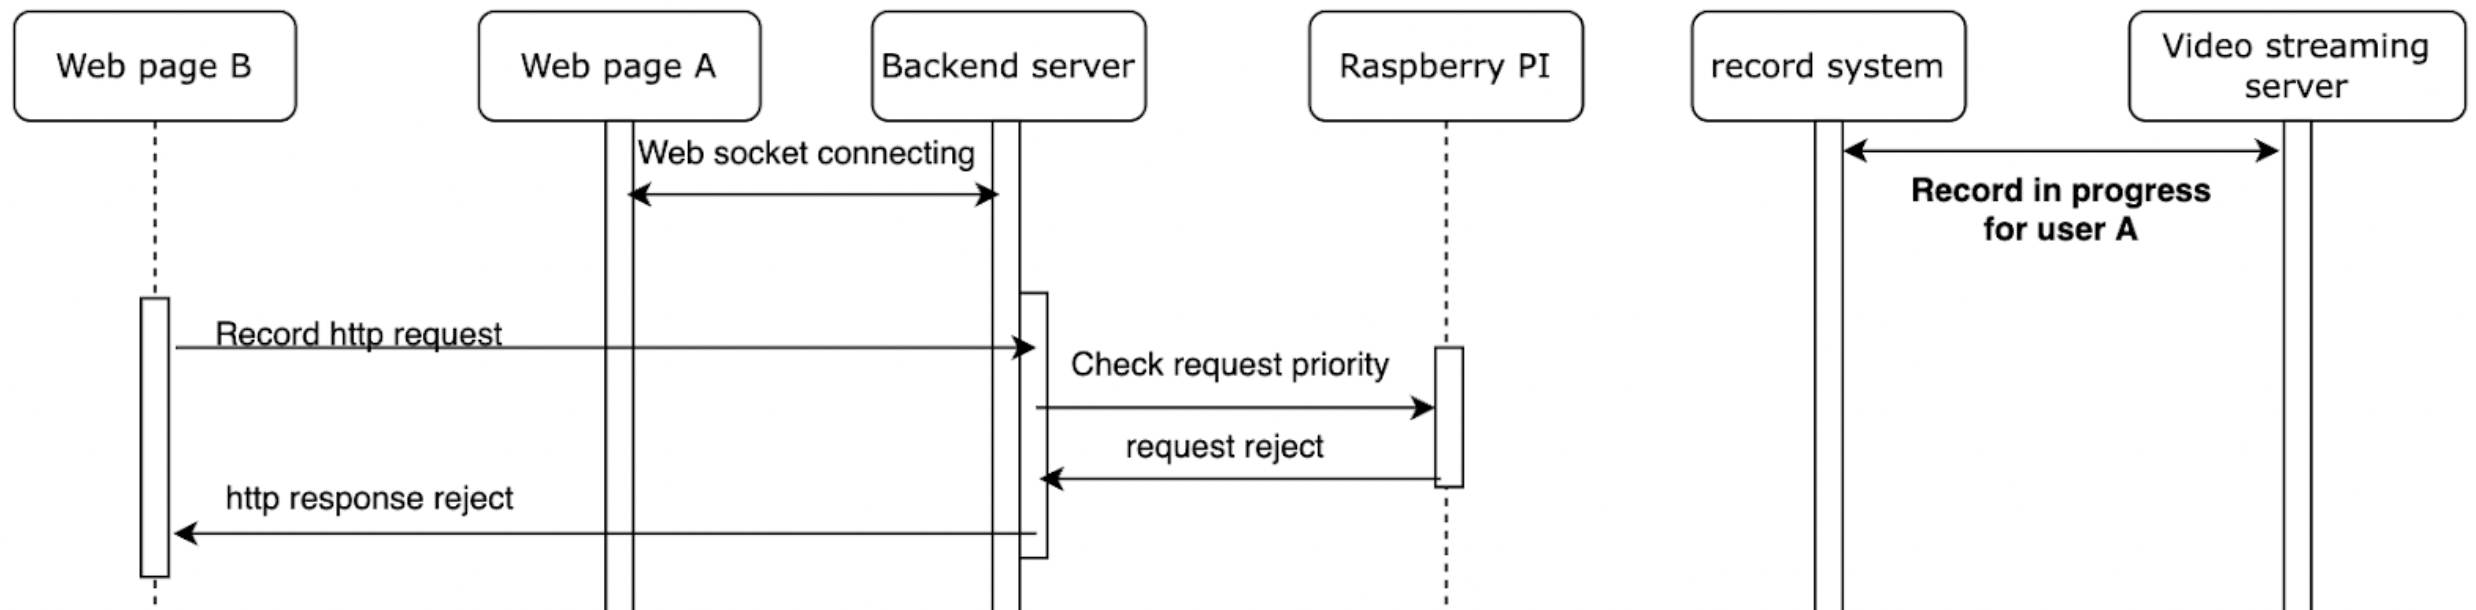
\includegraphics[width=\textwidth]{figsrc/preemptive-B-lower.png}
        \subcaption{User B with lower priority}
        \label{fig:preemptive-B-lower}
    \end{subfigure}

    \caption{Data flow of preemptive case}
    \label{fig:preemptive-sequence}
\end{figure}

We have shown how our system deal with crtical preemptive case. Next, we will explain detail of two main components in our system, raspberry PI and Recording server. 

% record system
\section{Structure of Recording server}
Recording server is the core component to perform recording task in the whole system. It is reponsible for recieving command from PI and recording live stream from Video streaming server. Our Recording server runs in AWS EC2~\cite{aws-ec2}. Operating System of EC2 VM is Ubuntu22.04. CPU is single Intel(R) Xeon(R) CPU E5-2676 v3 @ 2.40GH. RAM has size of 1 GB. Fig.~\ref{fig:recording-server-diagram} shows the architecture of record server. There are 3 components in it, receiver, master and slave. We will explain the feature of these 3 components. We use Master-Slave Replication to deal with different recording requests. Since Recording server may recieve multiple requests from different PI at the same time. It is important that Recording server is able to record multiple live streaming from Video streaming server simultaneously. 

\begin{figure}[H]
    \centering
    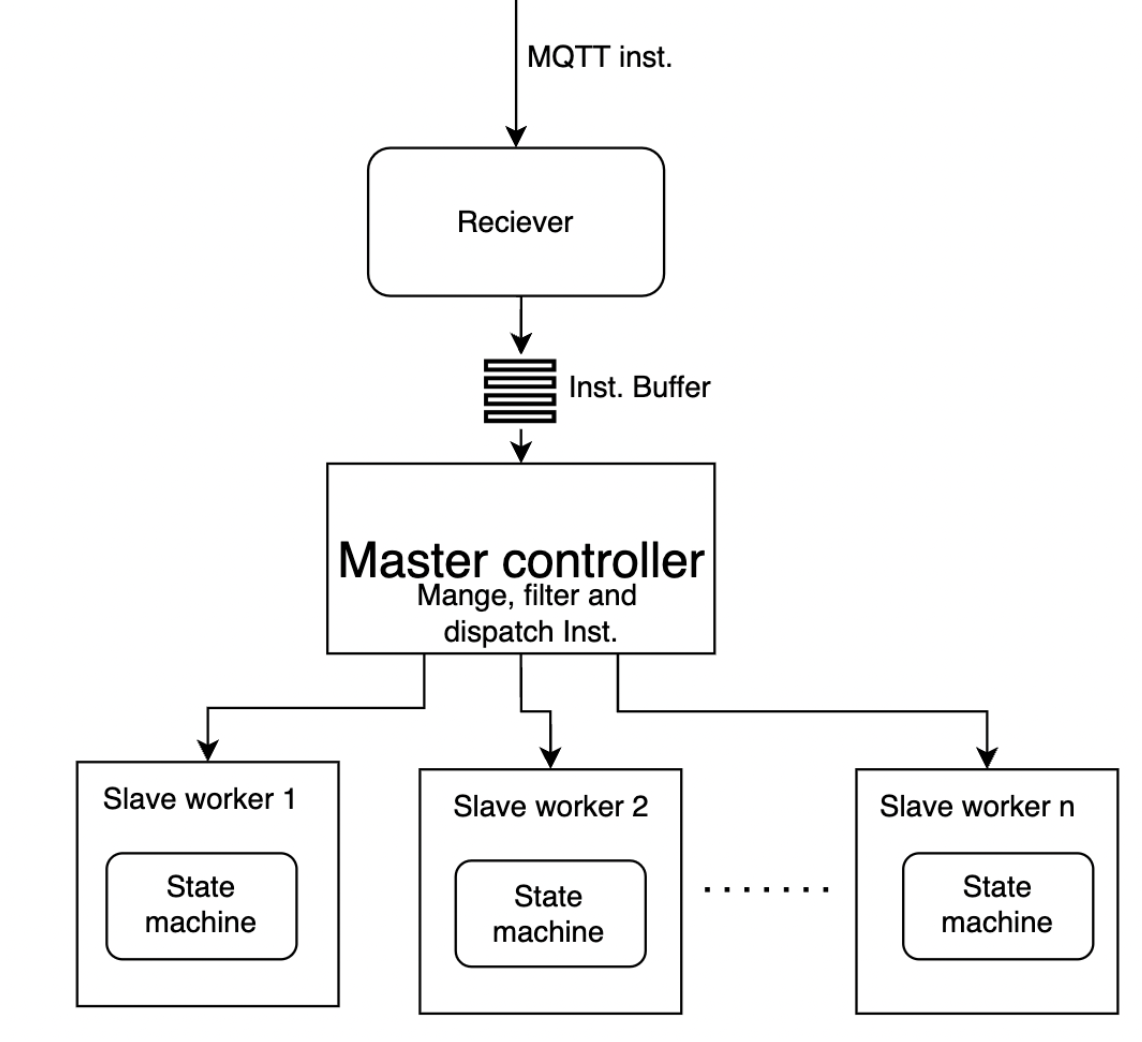
\includegraphics[width=\textwidth]{figsrc/recording-server-diagram.png}
    \caption{Structure of Recording server \label{fig:recording-server-diagram}}
\end{figure}

\subsection{Receiver}
Reciever is reponsible for getting command from PI which may locates at any experiment field. We implement reciever by paho-mqtt python package~\cite{paho-mqtt} to recieve MQTT message. Addtionally, we also implement a buffer to prevent message overflow.

\subsection{Master}
Master is responsible for managing the command recieved from PI. It is designed for tackling multiple recording request at the same time. If master recieves new request, it will create new slave to record new stream. If some slaves finish its tasks, master will terminate the slaves and release their resources.

\subsection{Slave}
Every single slave is responsible for recording one corresponding stream of camera as shown in Fig.~\ref{fig:recording-server-slave}. We use state machine to implement slave. As shown in Fig.~\ref{fig:recording-server-stg}, There are 4 states in state machine, S0 to S3. When entering a new state, slave will always inform PI to make sure that PI always knows the situation in Recording server. S0 is the initial state when the slave is created by master. It will start connecting to Video streaming server. When it finishes connection, it will inform PI that it is ready to record and switch to S2. S2 is stand by state, it will wait PI's command to shut down or start recording process. S1 is recording state that it will start to record the stream until time's up or stopped by user or replaced by other higher priority task. S3 is the termination state. It will disconnect with Video streaming server and free the resources. S1 and S2 will automatically terminate if they don't get command for a period of time.

\begin{figure}[H]
    \centering
    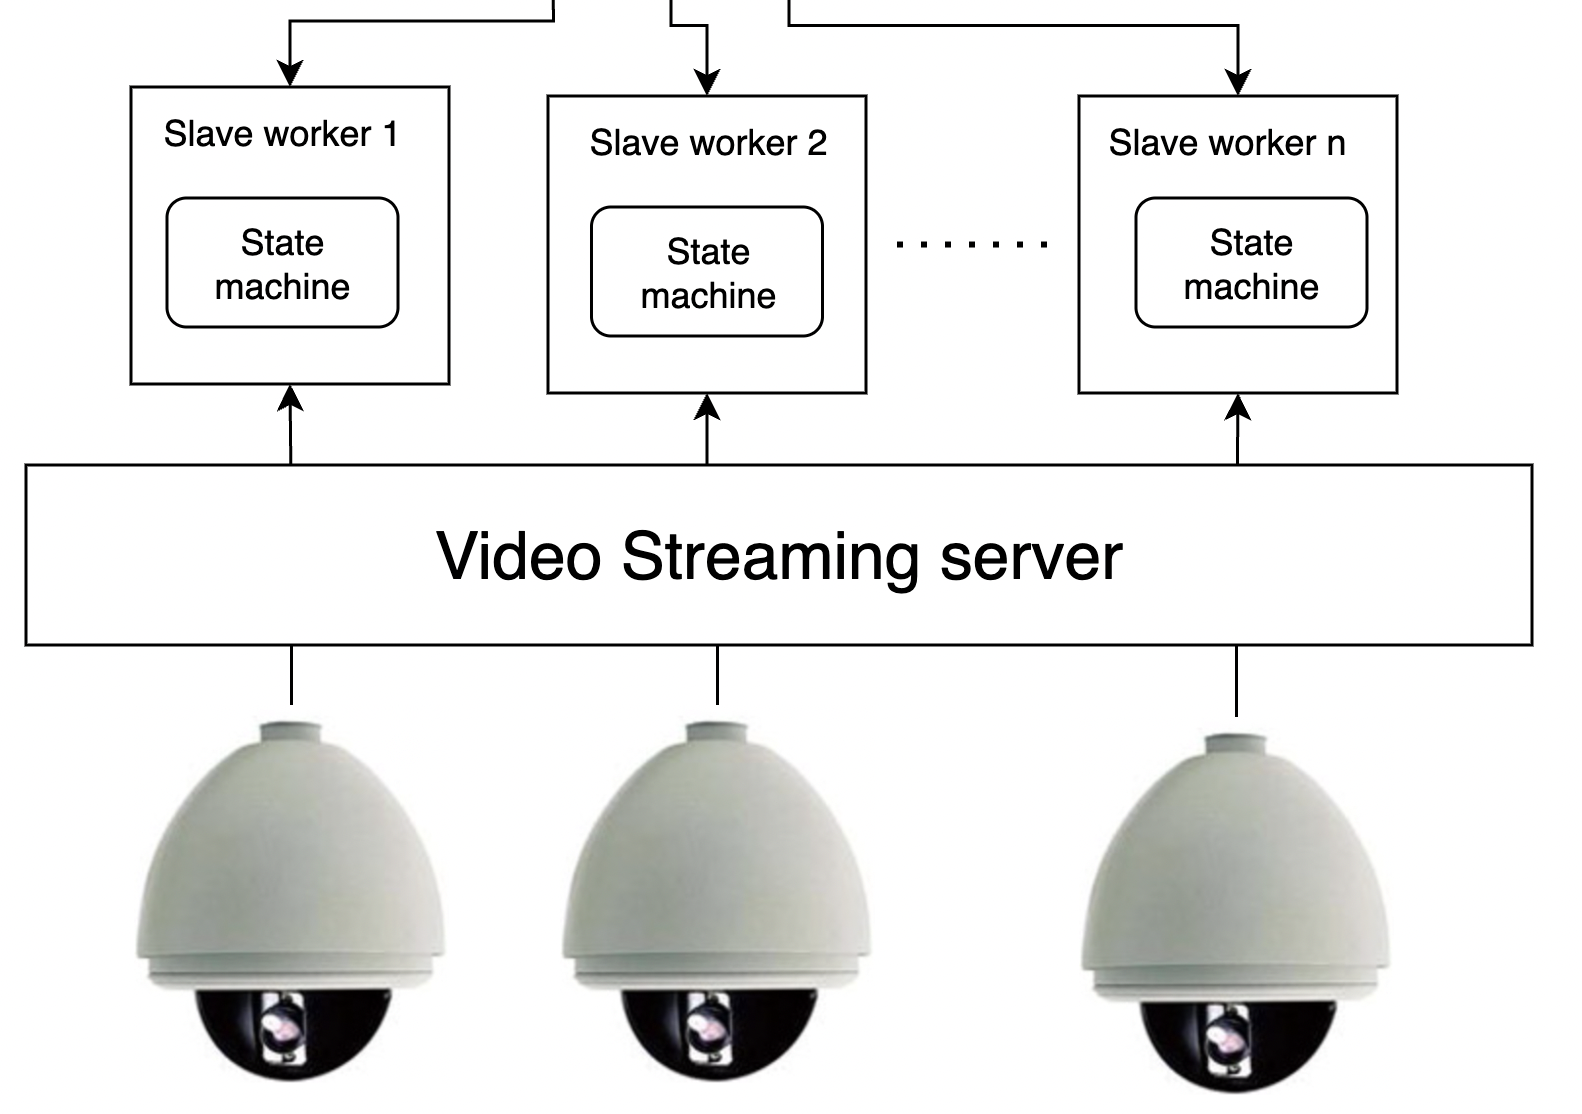
\includegraphics[width=\textwidth]{figsrc/recording-server-slave.png}
    \caption{Each slave records one independent stream\label{fig:recording-server-slave}}
\end{figure}


\begin{figure}[H]
    \centering
    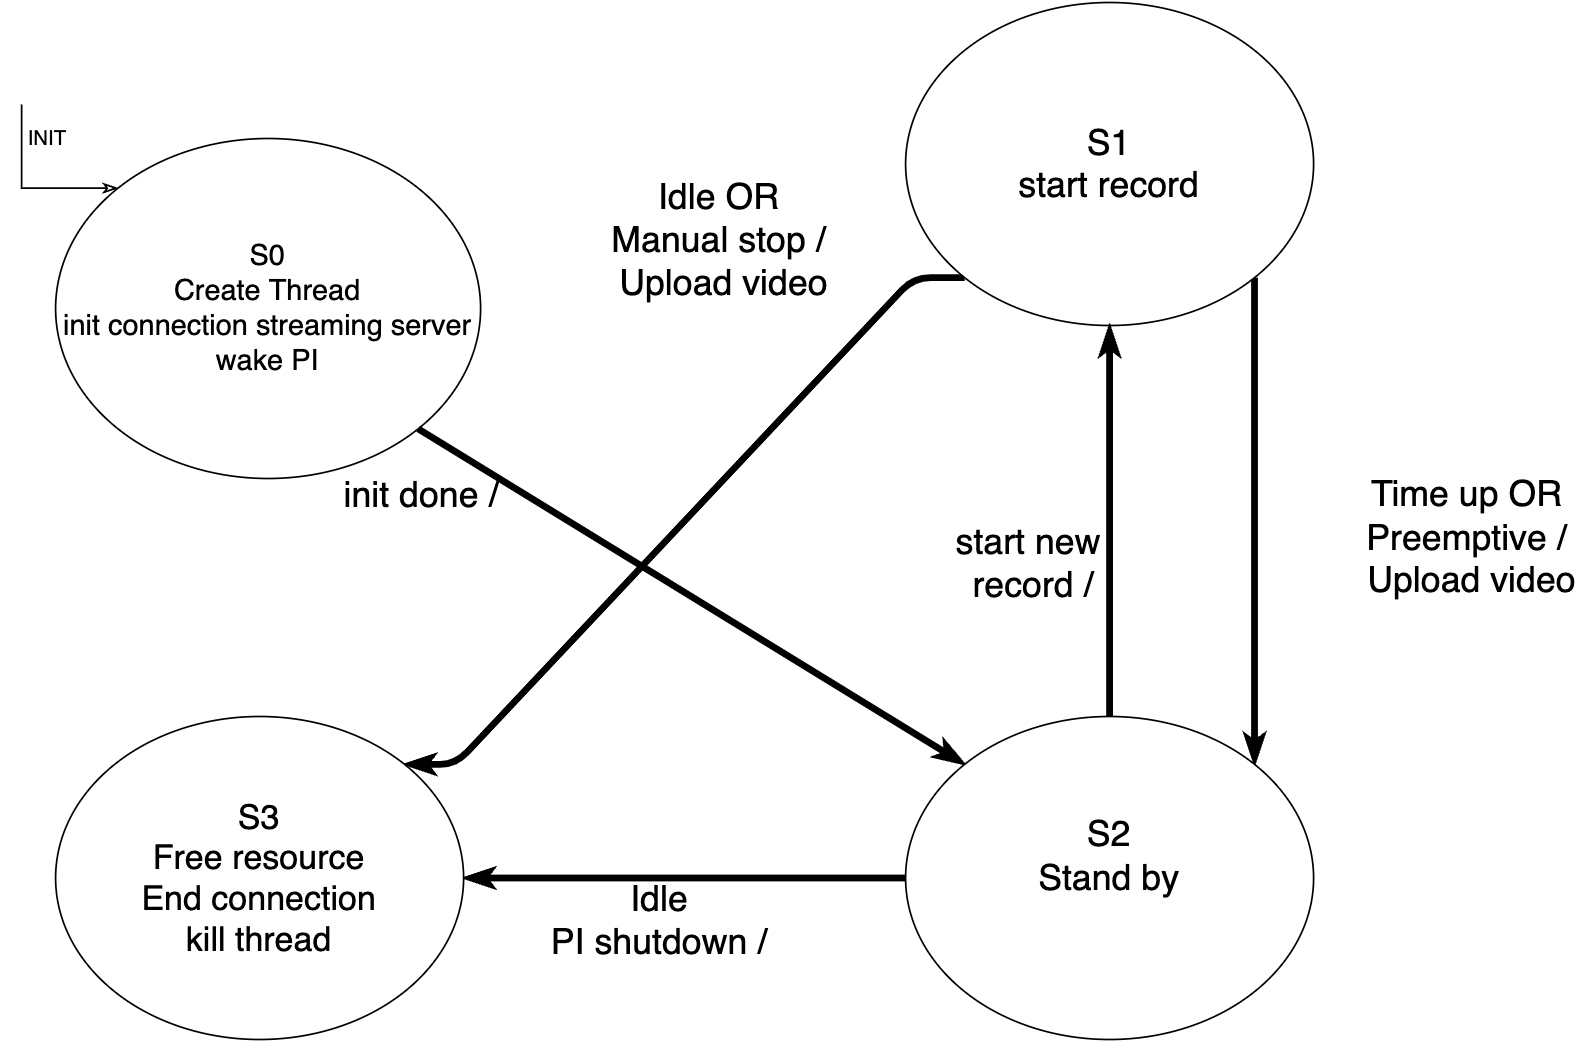
\includegraphics[width=\textwidth]{figsrc/recording-server-stg.png}
    \caption{State transition graph of state machine of slave\label{fig:recording-server-stg}}
\end{figure}

% PI
\section{Structure of Raspberry}
PI not only needs to recieve command from Front-end side but also has to coordinate with Recording server. Furthermore, PI even needs to deal with preeemptive case. It has to decide which task to execute or terminate. So in order to handle such complex situation, we propose a decision tree that is able to solve the problem as shown in Fig.~\ref{fig:pi-decision-tree}. We use decision tree to indicate how we manage the preemptive case and data between frontend and record server. It will determine how to deal with incoming message. For upper subtree, the message is come from Recording server. It indicates that which state the slave is currently at, so PI will know which command it shall send to Recording server next. If PI finds that the response from Recording server is invalid, it will order Recording server to teminate the slave. For lower subtree, it has three types of command, stop, check and create. Check command will respond to Front-end whether the new task has permission or not. Stop command will stop the recording process in manual case. Create command is more complex than previous two. It will first check whether there is a task which is currently occupying the corresponding camera stream or not. If Recording server is idle, PI will directly send create command to recording server; If Recording server is occupied, PI will check the priority between two task. If new task has lower priority, PI will ignore the new request; If new task has higher priority, PI will order recording server to terminate old task then send new command to execute new task.

\begin{figure}[H]
    \centering
    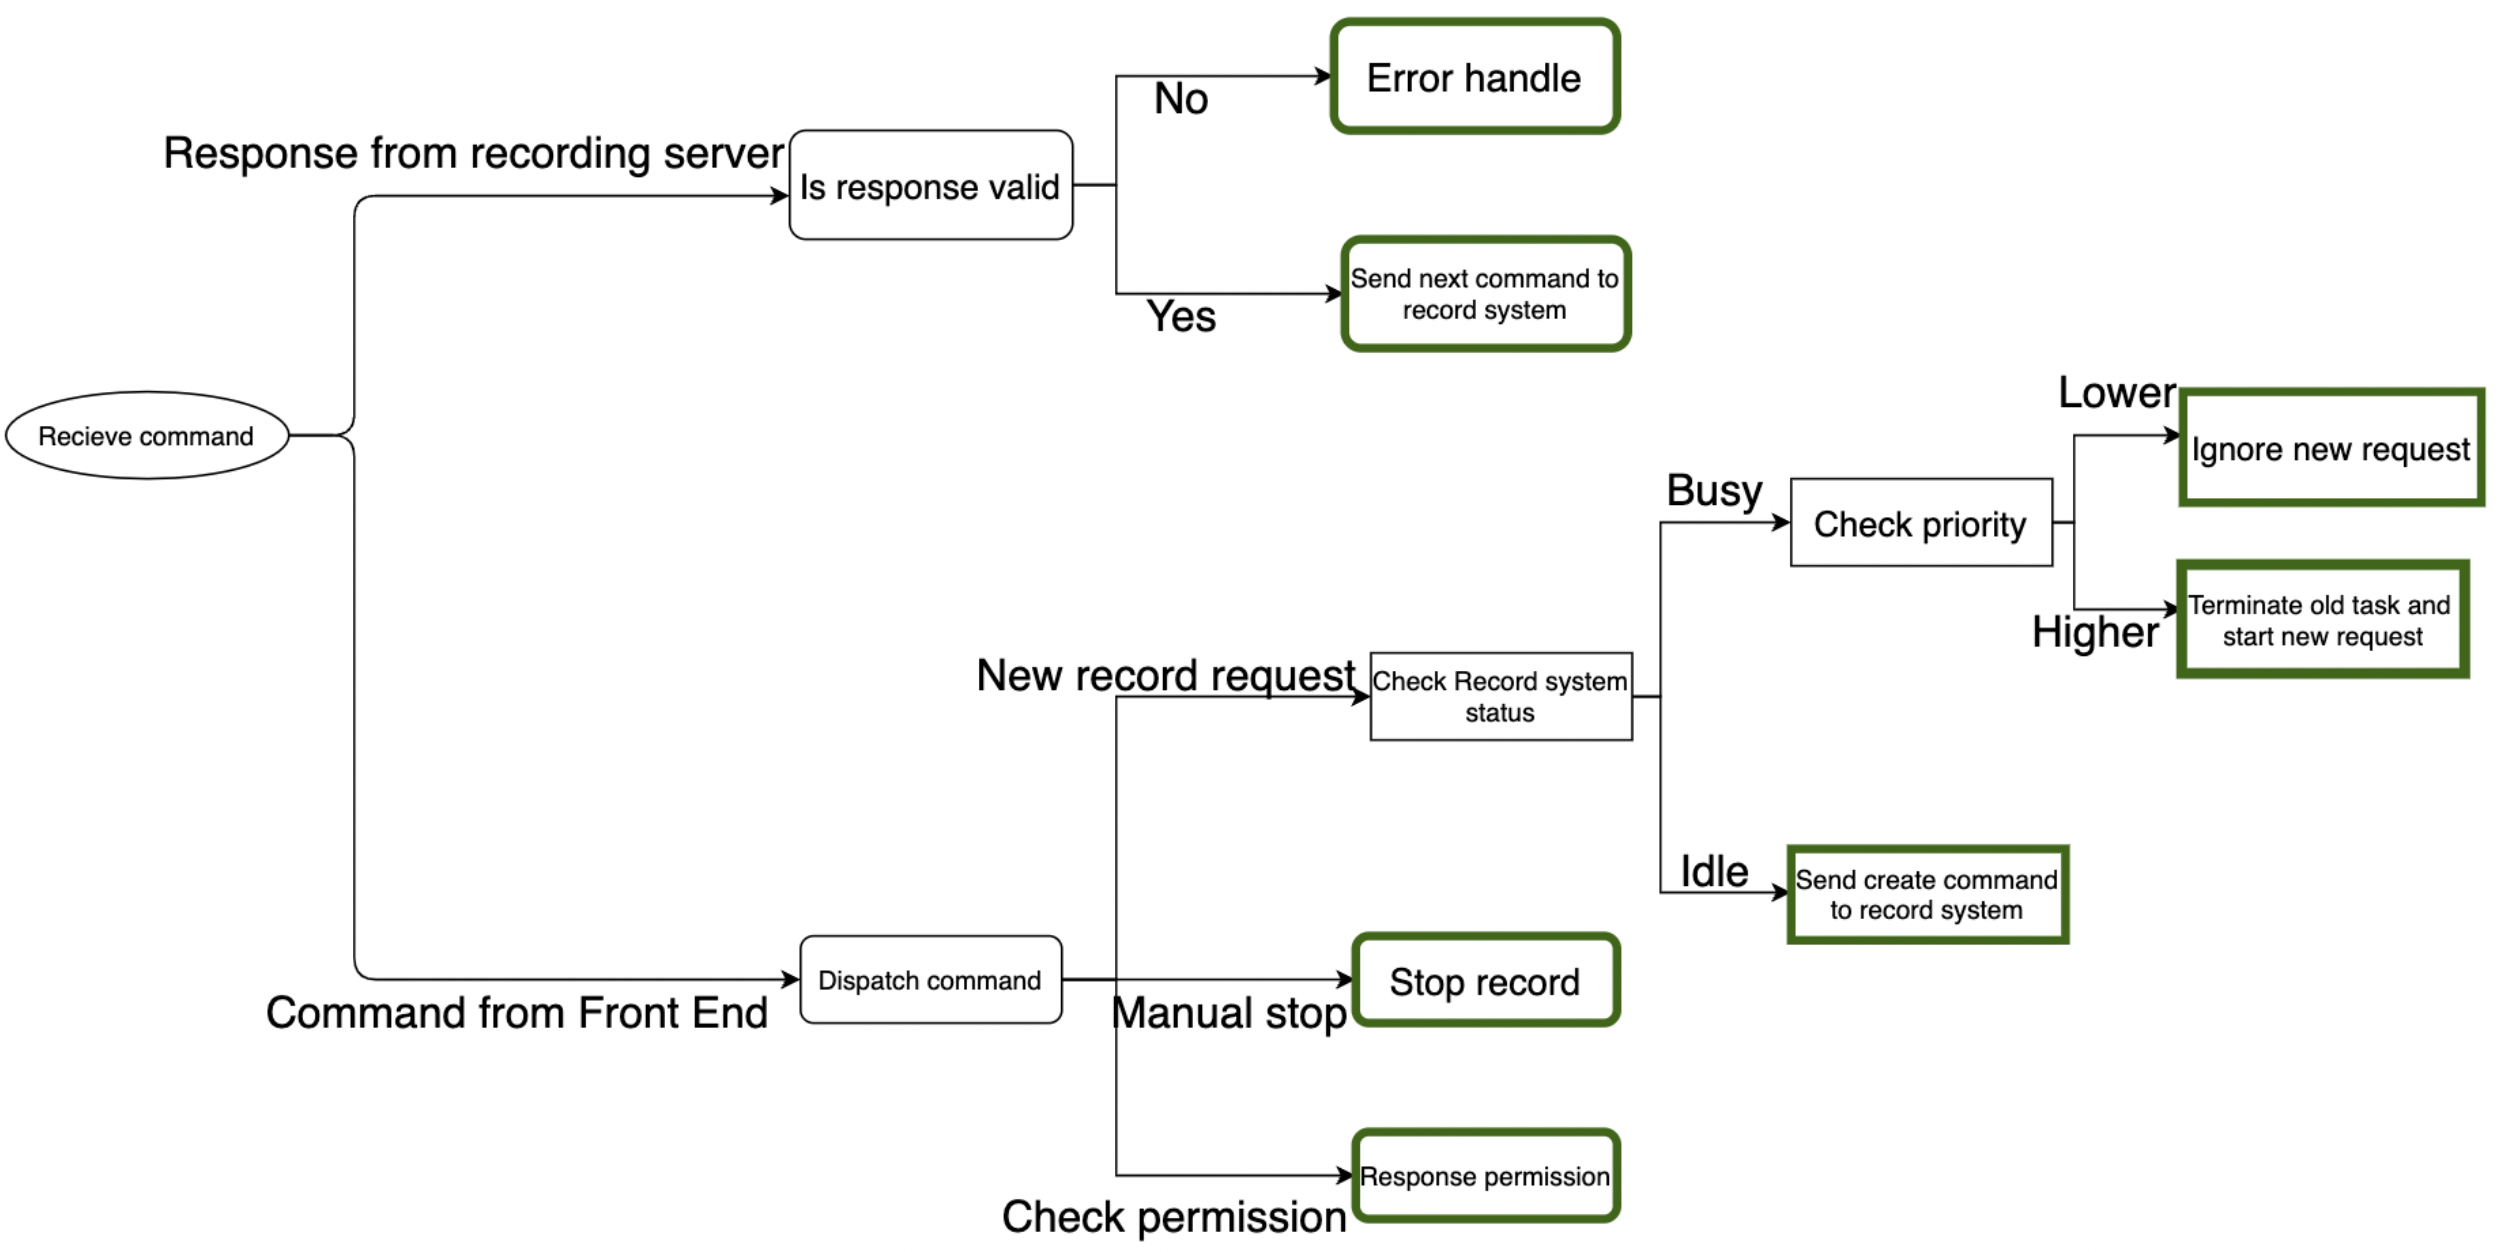
\includegraphics[width=\textwidth]{figsrc/pi-decision-tree.png}
    \caption{Decision tree of PI\label{fig:pi-decision-tree}}
\end{figure}